\documentclass[a4paper,12pt]{article}

\usepackage[utf8]{inputenc}
\usepackage[spanish]{babel}
\usepackage{amsmath, amssymb}
\usepackage{graphicx}
\usepackage{float}
\usepackage{booktabs}
\usepackage{xcolor}
\usepackage{listings}
\usepackage{caption}
\usepackage{fancyhdr}
\usepackage{hyperref}
\usepackage{tikz}

\hypersetup{
    colorlinks=true,
    linkcolor=blue,
    urlcolor=blue,
    pdftitle={Práctica 1 - Circuitos Combinacionales},
}

% === Definición de colores similares a Vivado ===
\definecolor{vivadoKeyword}{rgb}{0.6,0.0,0.6}
\definecolor{vivadoComment}{rgb}{0.0,0.5,0.0}
\definecolor{vivadoString}{rgb}{0.5,0.2,0.0}
\definecolor{vivadoBackground}{rgb}{0.97,0.97,0.97}

\lstdefinelanguage{VHDL}{
    morekeywords={library, use, entity, is, port, in, out, end, architecture, of, begin, signal, if, then, else, when, others, xor, and, or, not},
    sensitive=true,
    morecomment=[l]--,
    morestring=[b]",
}

\lstset{
    language=VHDL,
    backgroundcolor=\color{vivadoBackground},
    keywordstyle=\color{vivadoKeyword}\bfseries,
    commentstyle=\color{vivadoComment}\itshape,
    stringstyle=\color{vivadoString},
    basicstyle=\ttfamily\small,
    numbers=left,
    numberstyle=\tiny,
    numbersep=5pt,
    frame=single,
    breaklines=true,
    tabsize=2,
    captionpos=b
}

\title{Práctica N°1: Circuitos Combinacionales}
\date{}

\begin{document}
\maketitle
\tableofcontents
\newpage

\section{Objetivos}

\subsection*{Objetivo general}
Diseñar, describir en VHDL e implementar en una FPGA Nexys un circuito combinacional a partir de una expresión lógica dada, utilizando el entorno de desarrollo Vivado y aplicando correctamente la lógica booleana.

\subsection*{Objetivos específicos}
\begin{itemize}
    \item Analizar y expresar algebraicamente la función lógica: \( Q = (A \cdot \overline{B}) \ XOR \ \overline{(C + D)} \).
    \item Elaborar la tabla de verdad correspondiente a la función dada.
    \item Describir el circuito mediante código VHDL estructurado, verificando su sintaxis y lógica.
    \item Asignar correctamente las señales de entrada/salida a los pines de la FPGA usando un archivo de restricciones \texttt{.xdc}.
    \item Sintetizar, implementar y programar el circuito en la tarjeta Nexys desde Vivado.
    \item Validar el comportamiento lógico del diseño en la placa, verificando que la salida coincida con lo esperado en la tabla de verdad.
\end{itemize}

\section{Ecuación}

La función lógica a implementar es:

\[
Q = (A \cdot \overline{B}) \ XOR \ \overline{(C + D)}
\]

\section{Tabla de Verdad}

La siguiente tabla muestra el desarrollo paso a paso de la función lógica:

\[
Q = (A \cdot \overline{B}) \ XOR \ \overline{(C + D)}
\]

\begin{table}[H]
\centering
\renewcommand{\arraystretch}{1.2}
\begin{tabular}{cccc|c|c|c|c|c}
\toprule
A & B & C & D & $\overline{B}$ & $A \cdot \overline{B}$ & $C + D$ & $\overline{(C + D)}$ & $Q$ \\
\midrule
0 & 0 & 0 & 0 & 1 & 0 & 0 & 1 & 1 \\
0 & 0 & 0 & 1 & 1 & 0 & 1 & 0 & 0 \\
0 & 0 & 1 & 0 & 1 & 0 & 1 & 0 & 0 \\
0 & 0 & 1 & 1 & 1 & 0 & 1 & 0 & 0 \\
0 & 1 & 0 & 0 & 0 & 0 & 0 & 1 & 1 \\
0 & 1 & 0 & 1 & 0 & 0 & 1 & 0 & 0 \\
0 & 1 & 1 & 0 & 0 & 0 & 1 & 0 & 0 \\
0 & 1 & 1 & 1 & 0 & 0 & 1 & 0 & 0 \\
1 & 0 & 0 & 0 & 1 & 1 & 0 & 1 & 0 \\
1 & 0 & 0 & 1 & 1 & 1 & 1 & 0 & 1 \\
1 & 0 & 1 & 0 & 1 & 1 & 1 & 0 & 1 \\
1 & 0 & 1 & 1 & 1 & 1 & 1 & 0 & 1 \\
1 & 1 & 0 & 0 & 0 & 0 & 0 & 1 & 1 \\
1 & 1 & 0 & 1 & 0 & 0 & 1 & 0 & 0 \\
1 & 1 & 1 & 0 & 0 & 0 & 1 & 0 & 0 \\
1 & 1 & 1 & 1 & 0 & 0 & 1 & 0 & 0 \\
\bottomrule
\end{tabular}
\caption{Evaluación paso a paso de la expresión lógica combinacional}
\end{table}

\noindent
\textbf{Interpretación:} Esta tabla detalla cada componente lógico intermedio involucrado en la evaluación de \( Q \). La negación de \( B \) y la suma lógica \( C + D \) permiten construir progresivamente la salida deseada. Esto no solo facilita la depuración y validación del circuito, sino que también entrena al estudiante a leer y descomponer funciones booleanas complejas, una habilidad clave en el diseño digital.


\newpage

\section{Descripción del circuito en VHDL}

\subsection{Creación del proyecto}

Para comenzar con la implementación del circuito combinacional, se debe crear un nuevo proyecto en Vivado. El procedimiento es el siguiente:

\begin{enumerate}
    \item Abrir Vivado y seleccionar \textbf{Create Project}.

    \begin{figure}[H]
    \centering
    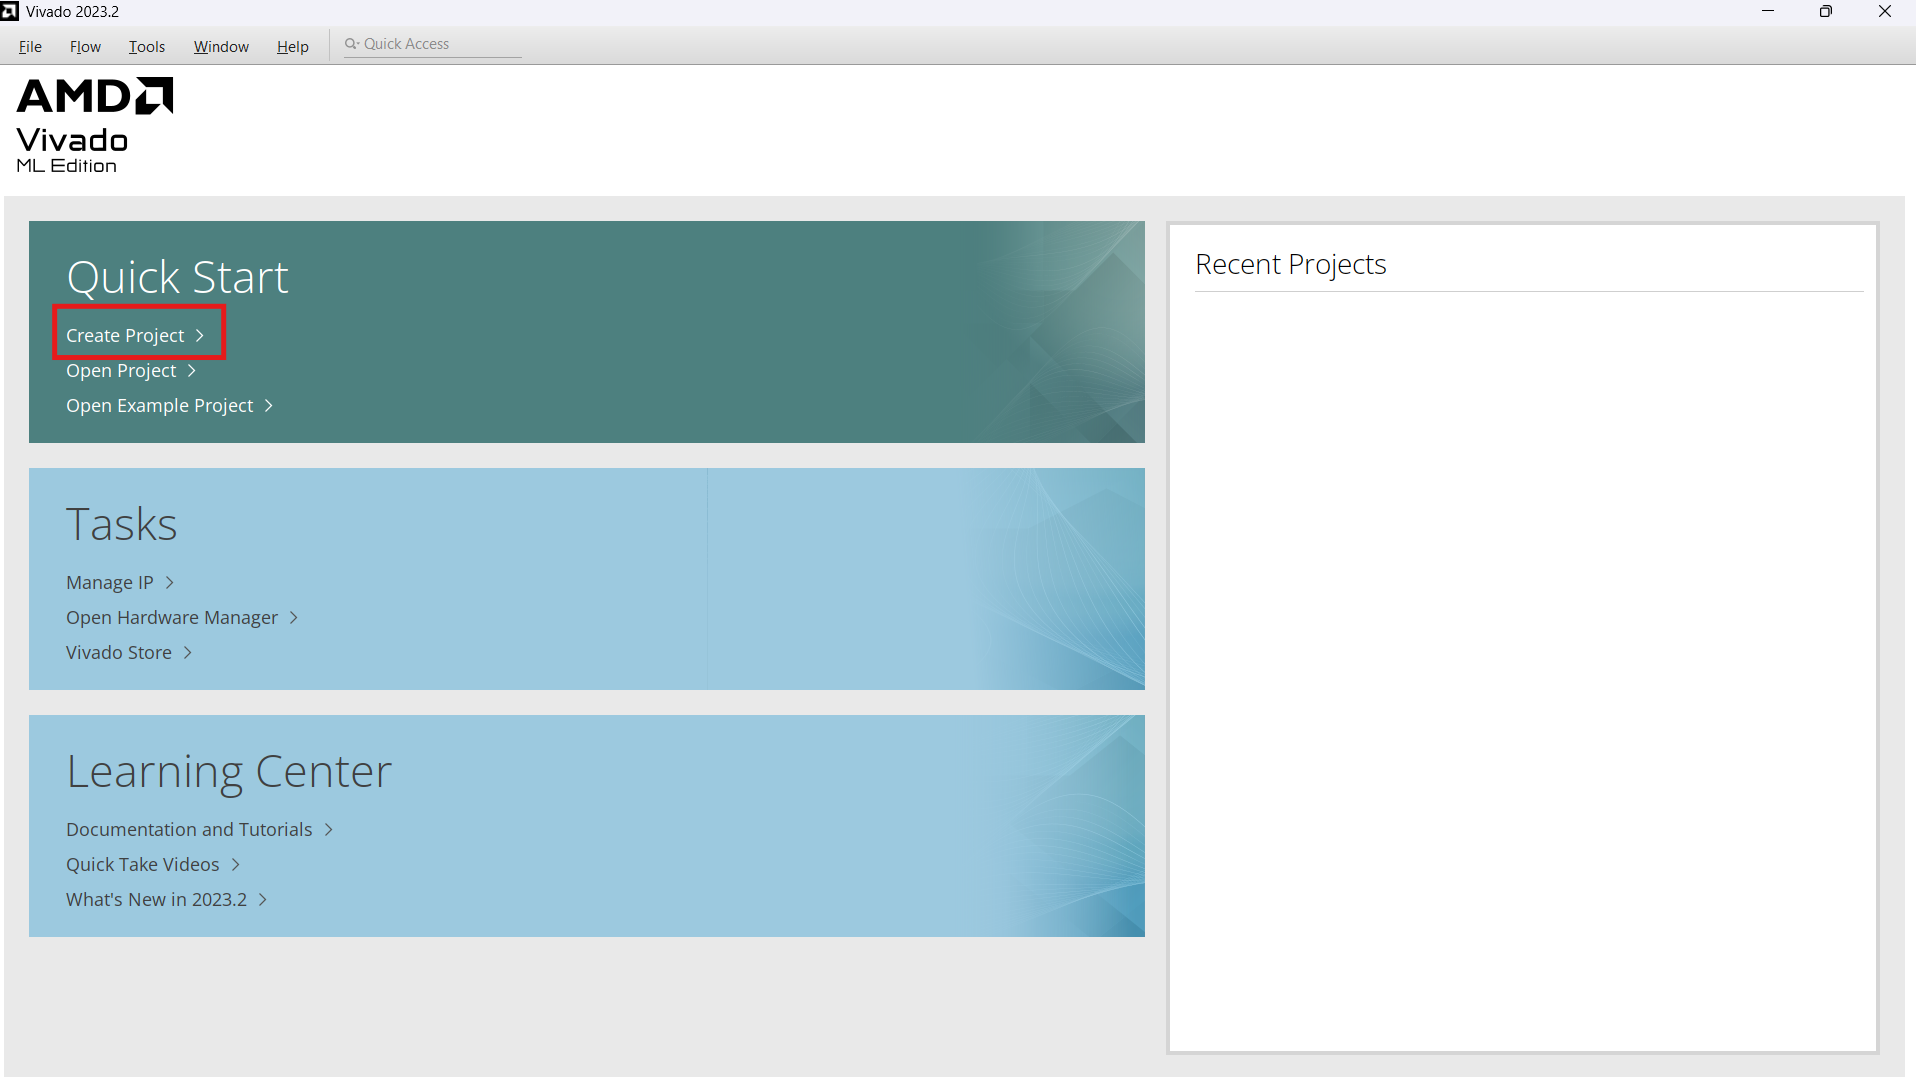
\includegraphics[width=0.8\textwidth]{Creacion_Proyecto/Crear_proyecto.png}
    \caption{Ventana de Inicializacion de Vivado para crear el proyecto.}
    \label{fig:Inicio}
    \end{figure}

    
    \item Asignar un nombre representativo al proyecto (por ejemplo, \\ \texttt{P1circuitocombinacional}) y definir la ubicación donde se guardará.

    \begin{figure}[H]
    \centering
    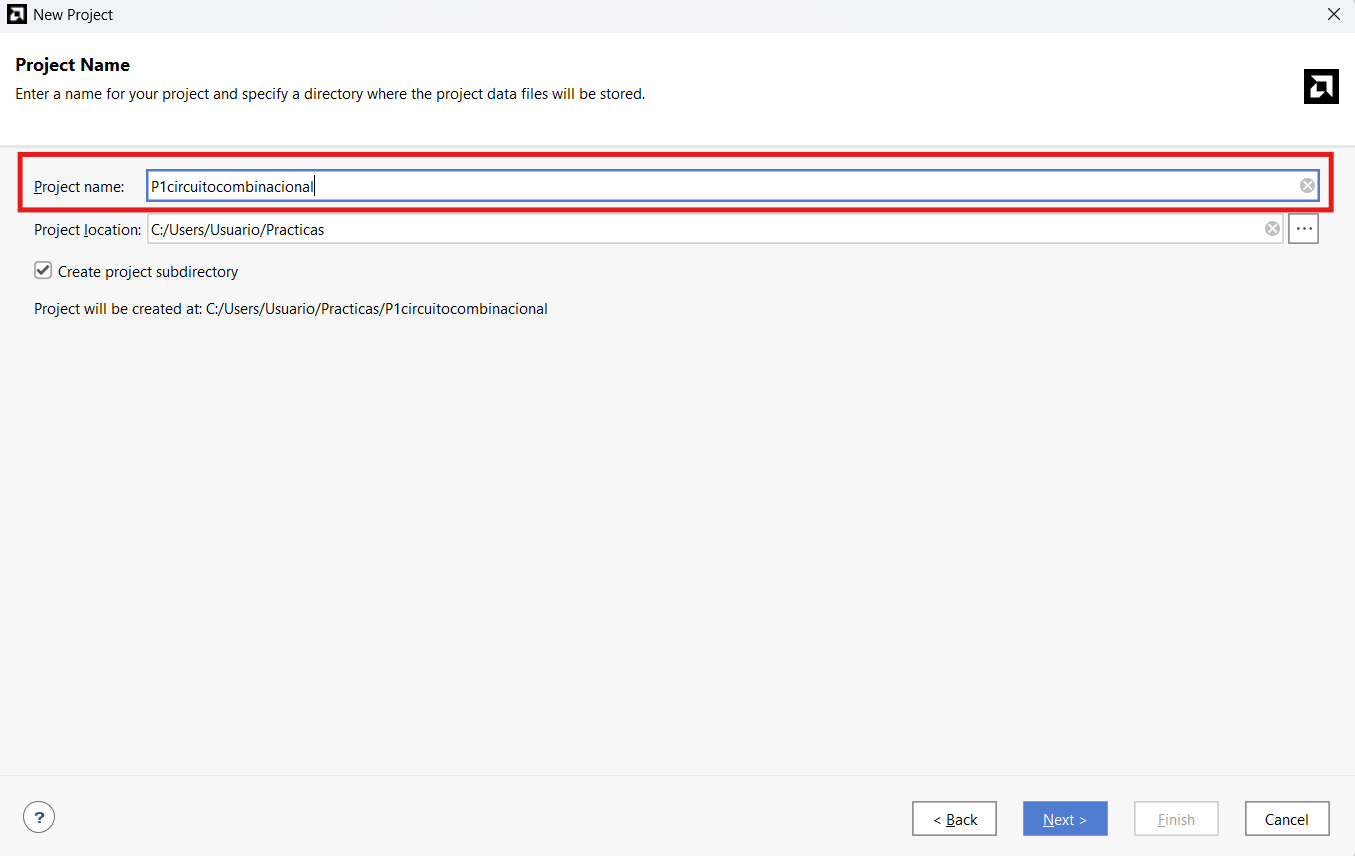
\includegraphics[width=0.8\textwidth]{Creacion_Proyecto/Nombre_proyecto.png}
    \caption{Nombre del proyecto.}
    \label{fig:nombre}
    \end{figure}

    \item En el asistente, seleccionar \textbf{RTL Project}.

    \begin{figure}[H]
    \centering
    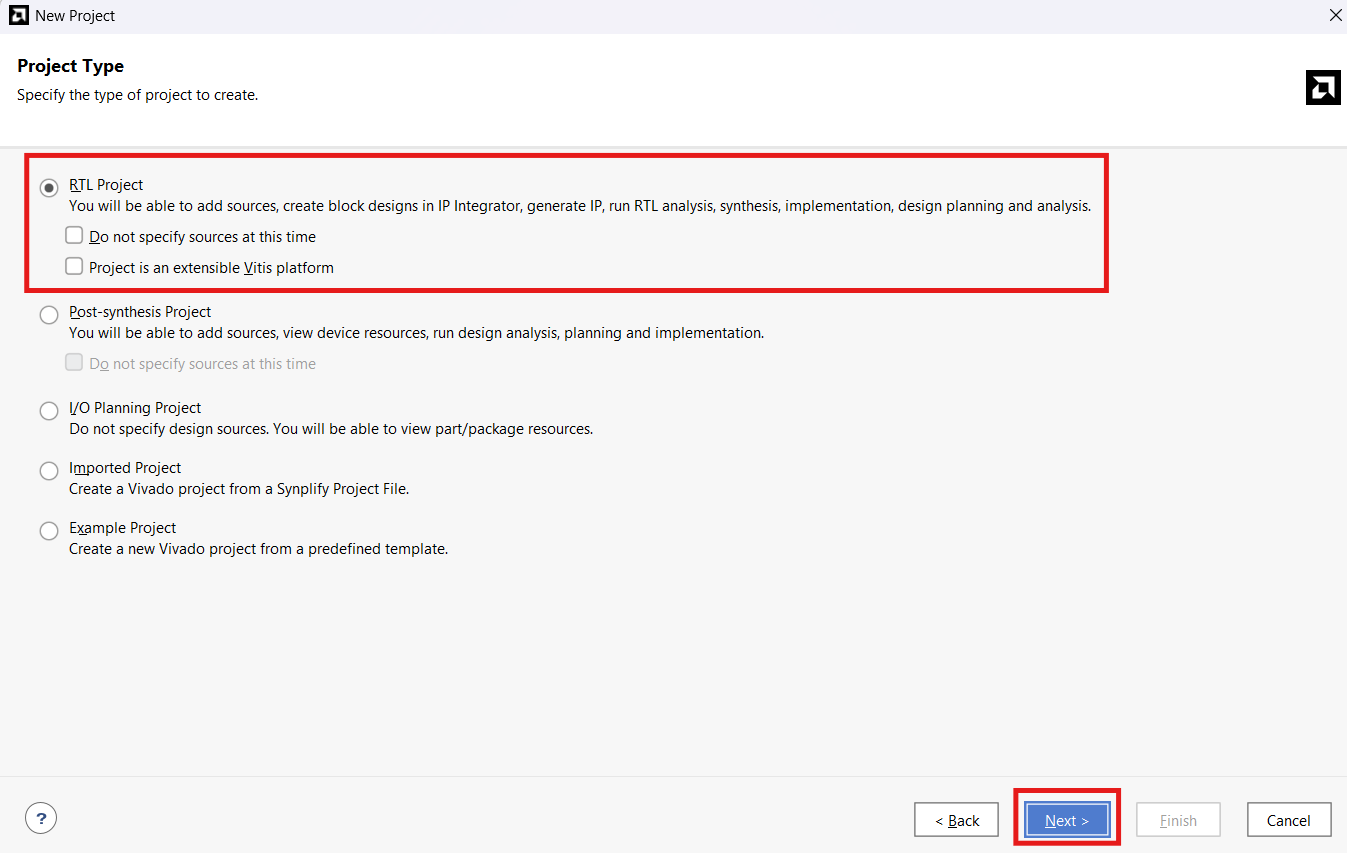
\includegraphics[width=0.8\textwidth]{Creacion_Proyecto/Tipo_proyecto.png}
    \caption{Tipo de proyecto creado.}
    \label{fig:RTL}
    \end{figure}

    \item A continuación, en el menú de recursos, debemos revisar las opciones de \textbf{Target Language:} y \textbf{Simulator Language:} ambas deben estar en la opción \textbf{VHDL}

    \begin{figure}[H]
    \centering
    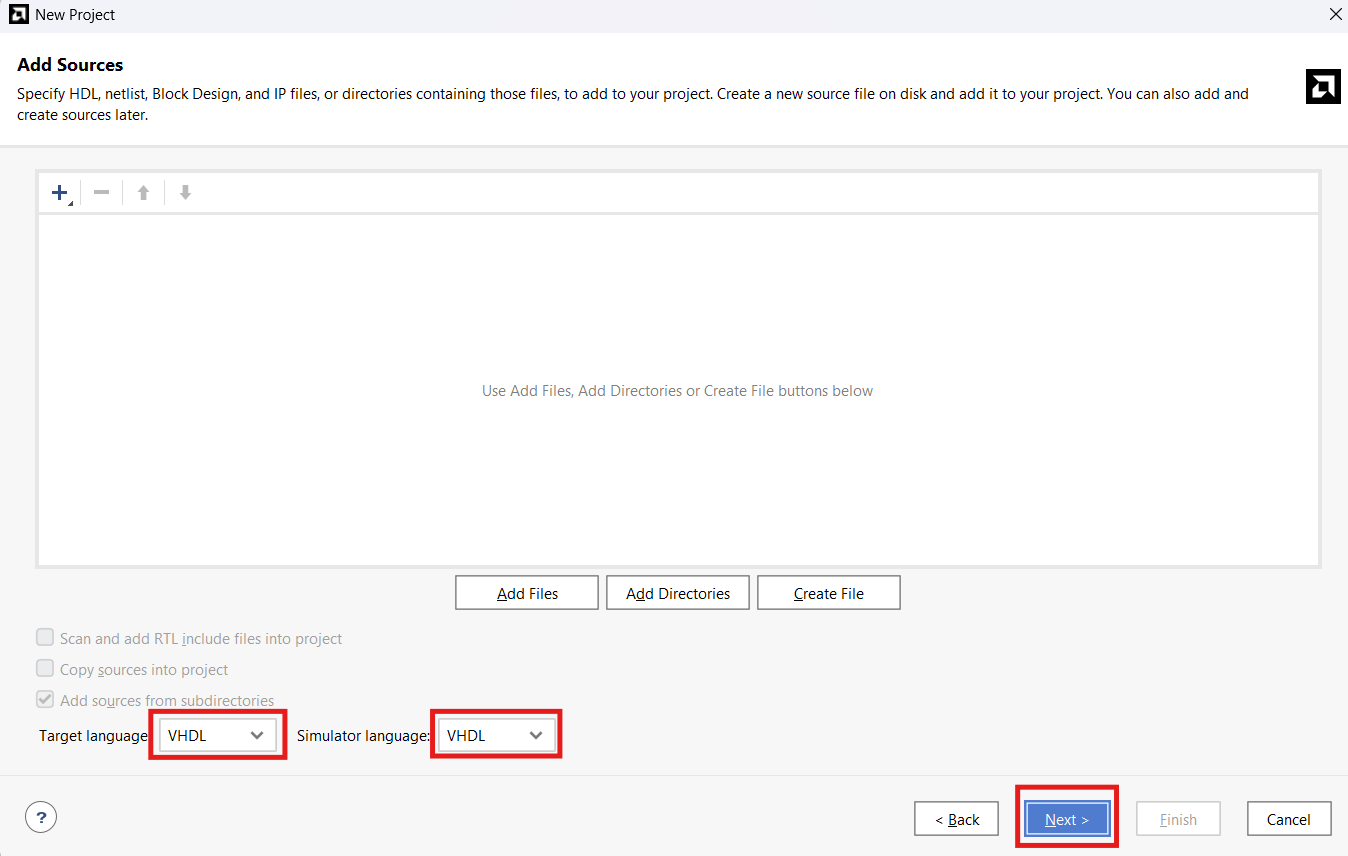
\includegraphics[width=0.8\textwidth]{Creacion_Proyecto/Recursos_proyecto.png}
    \caption{Recursos del proyecto.}
    \label{fig:recursos}
    \end{figure}

    \newpage

    \item El siguiente menú de configuraciones es el de restricciones, en este no vamos a configurar nada, dirigiéndonos al siguiente paso

    \begin{figure}[H]
    \centering
    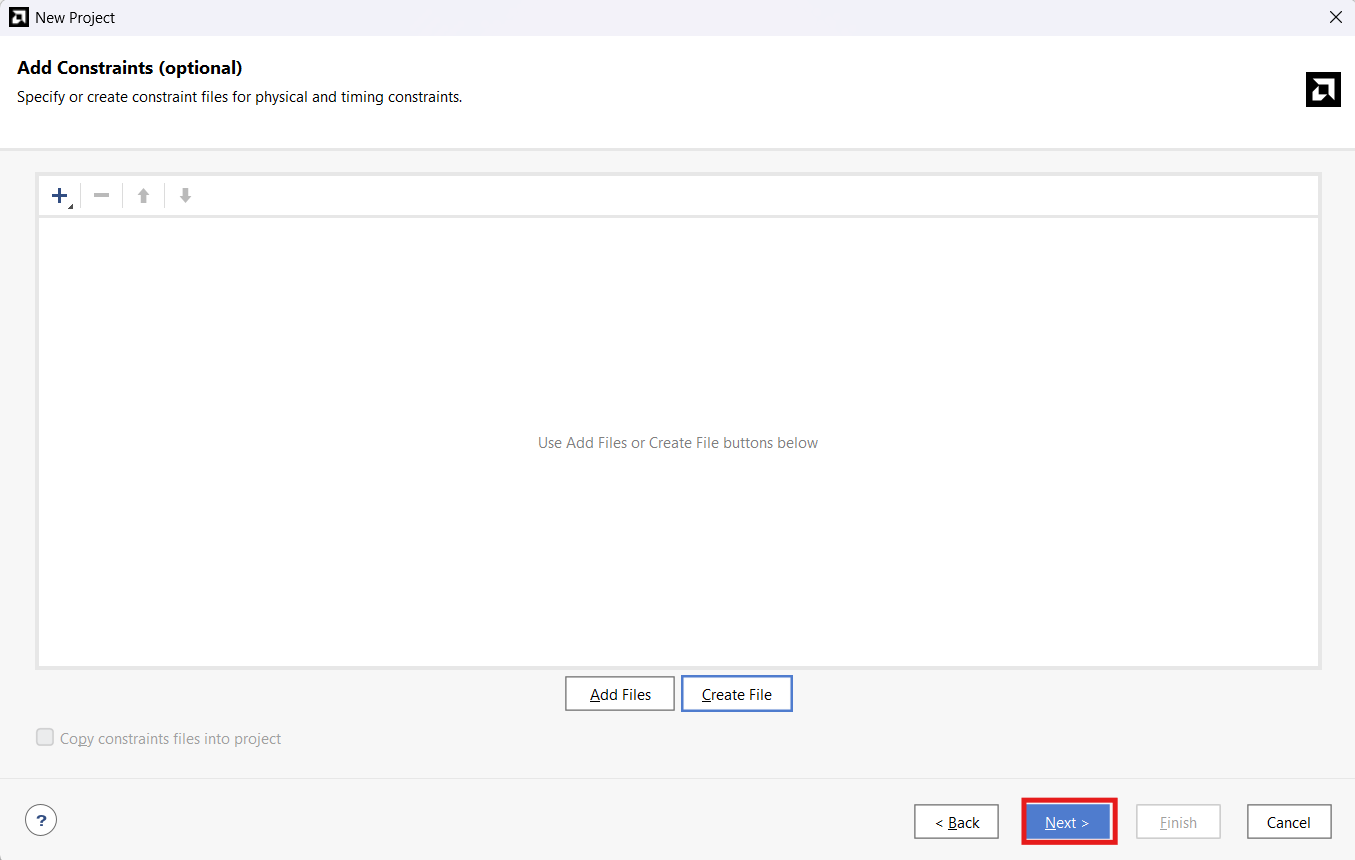
\includegraphics[width=0.8\textwidth]{Creacion_Proyecto/Constraints_proyecto.png}
    \caption{Restricciones del proyecto.}
    \label{fig:restricciones}
    \end{figure}

    \item En la sección de selección de la tarjeta, buscar y elegir el modelo correspondiente. Para esta práctica se utiliza:

    \begin{center}
        \texttt{NEXYS DDR4}
    \end{center}

    Esta corresponde a la FPGA que integra la tarjeta Nexys DDR4. Para ello nos dirigimos al menú de Boards, en este utilizando el buscador, se introduce el código de la placa. En caso que no este descargado, la comuna "status" se encontrara con un símbolo de descarga.

    \begin{figure}[H]
    \centering
    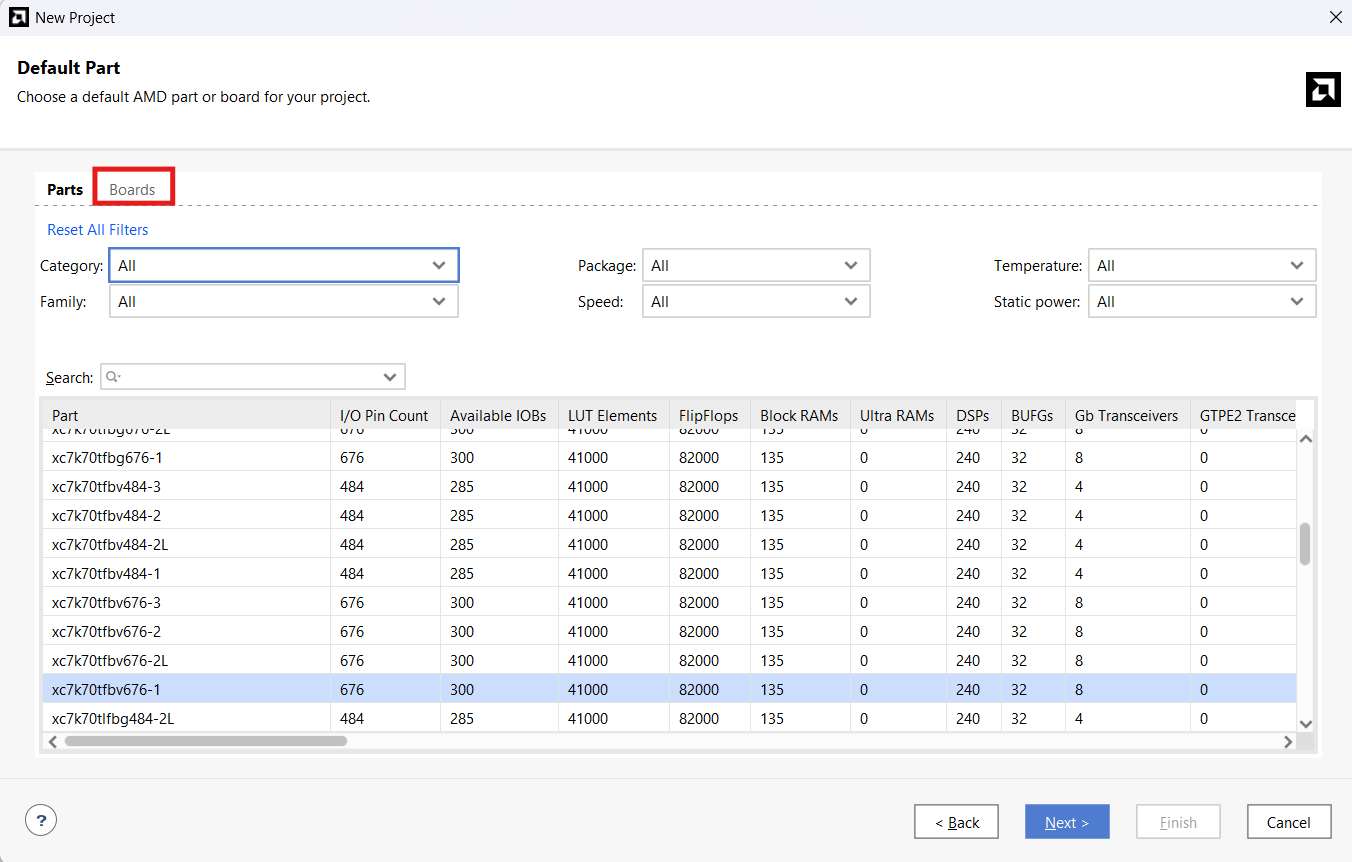
\includegraphics[width=0.8\textwidth]{Creacion_Proyecto/Board_proyecto.png}
    \caption{Acceso al menú de placas disponibles.}
    \label{fig:placas}
    \end{figure}

    \begin{figure}[H]
    \centering
    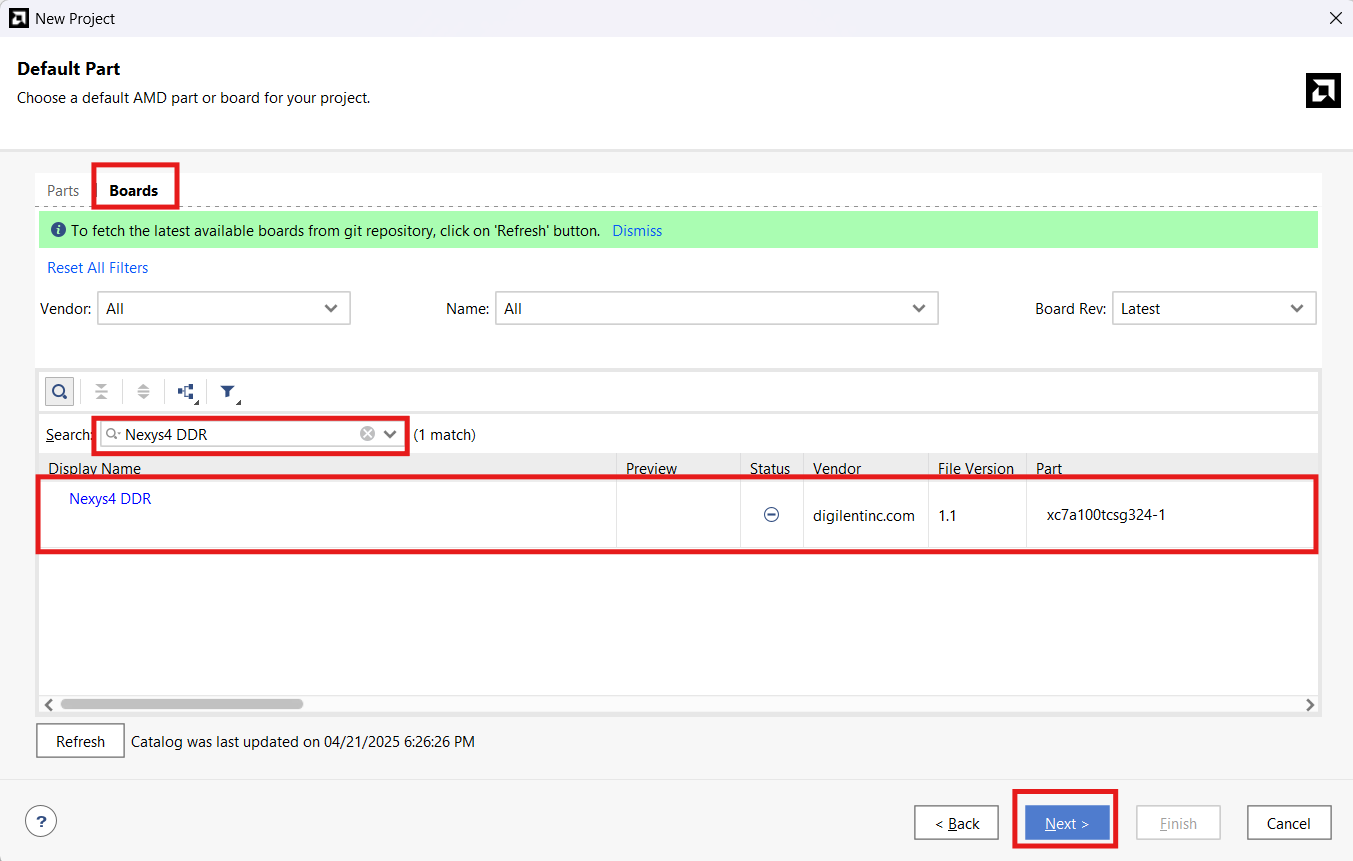
\includegraphics[width=0.8\textwidth]{Creacion_Proyecto/Placa_Proyecto.png}
    \caption{Seleccion de la placa.}
    \label{fig:seleccion}
    \end{figure}

    \newpage

    \item Una vez terminada esta configuración, se debe finalizar la creación del proyecto, con la opción \textbf{Finish}, con ello completamos este proceso.

    \begin{figure}[H]
    \centering
    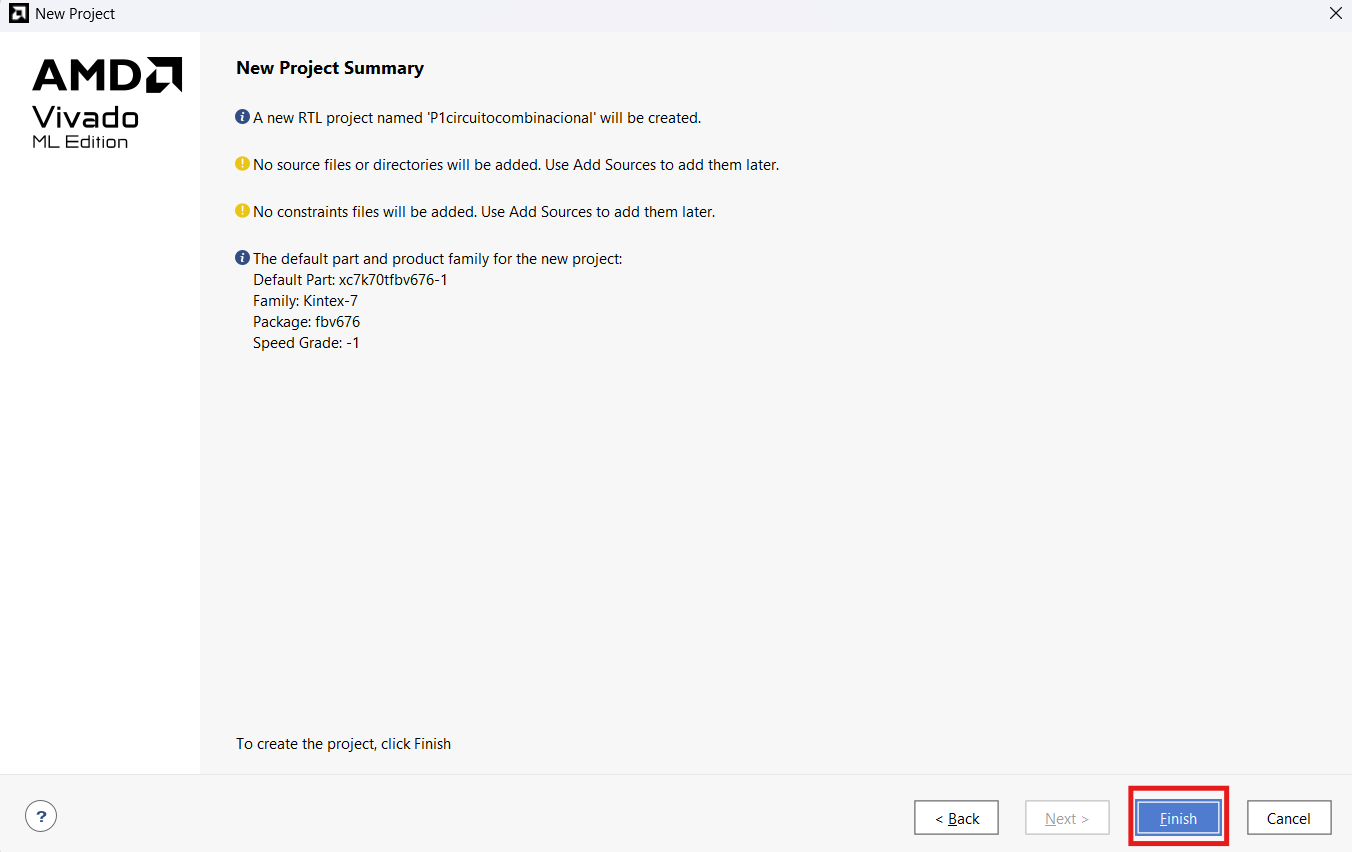
\includegraphics[width=0.8\textwidth]{Creacion_Proyecto/Finish_proyecto.png}
    \caption{Etapa final de la creación del proyecto.}
    \label{fig:final}
    \end{figure}

    \item Con el proyecto creado, el siguiente paso es crear el archivo \textbf{.vhd} en el cual se programará el codigo con la logica requerida, para ello se debe utilizar el simbolo '+' ubicado en el menú de recursos.

    \begin{figure}[H]
    \centering
    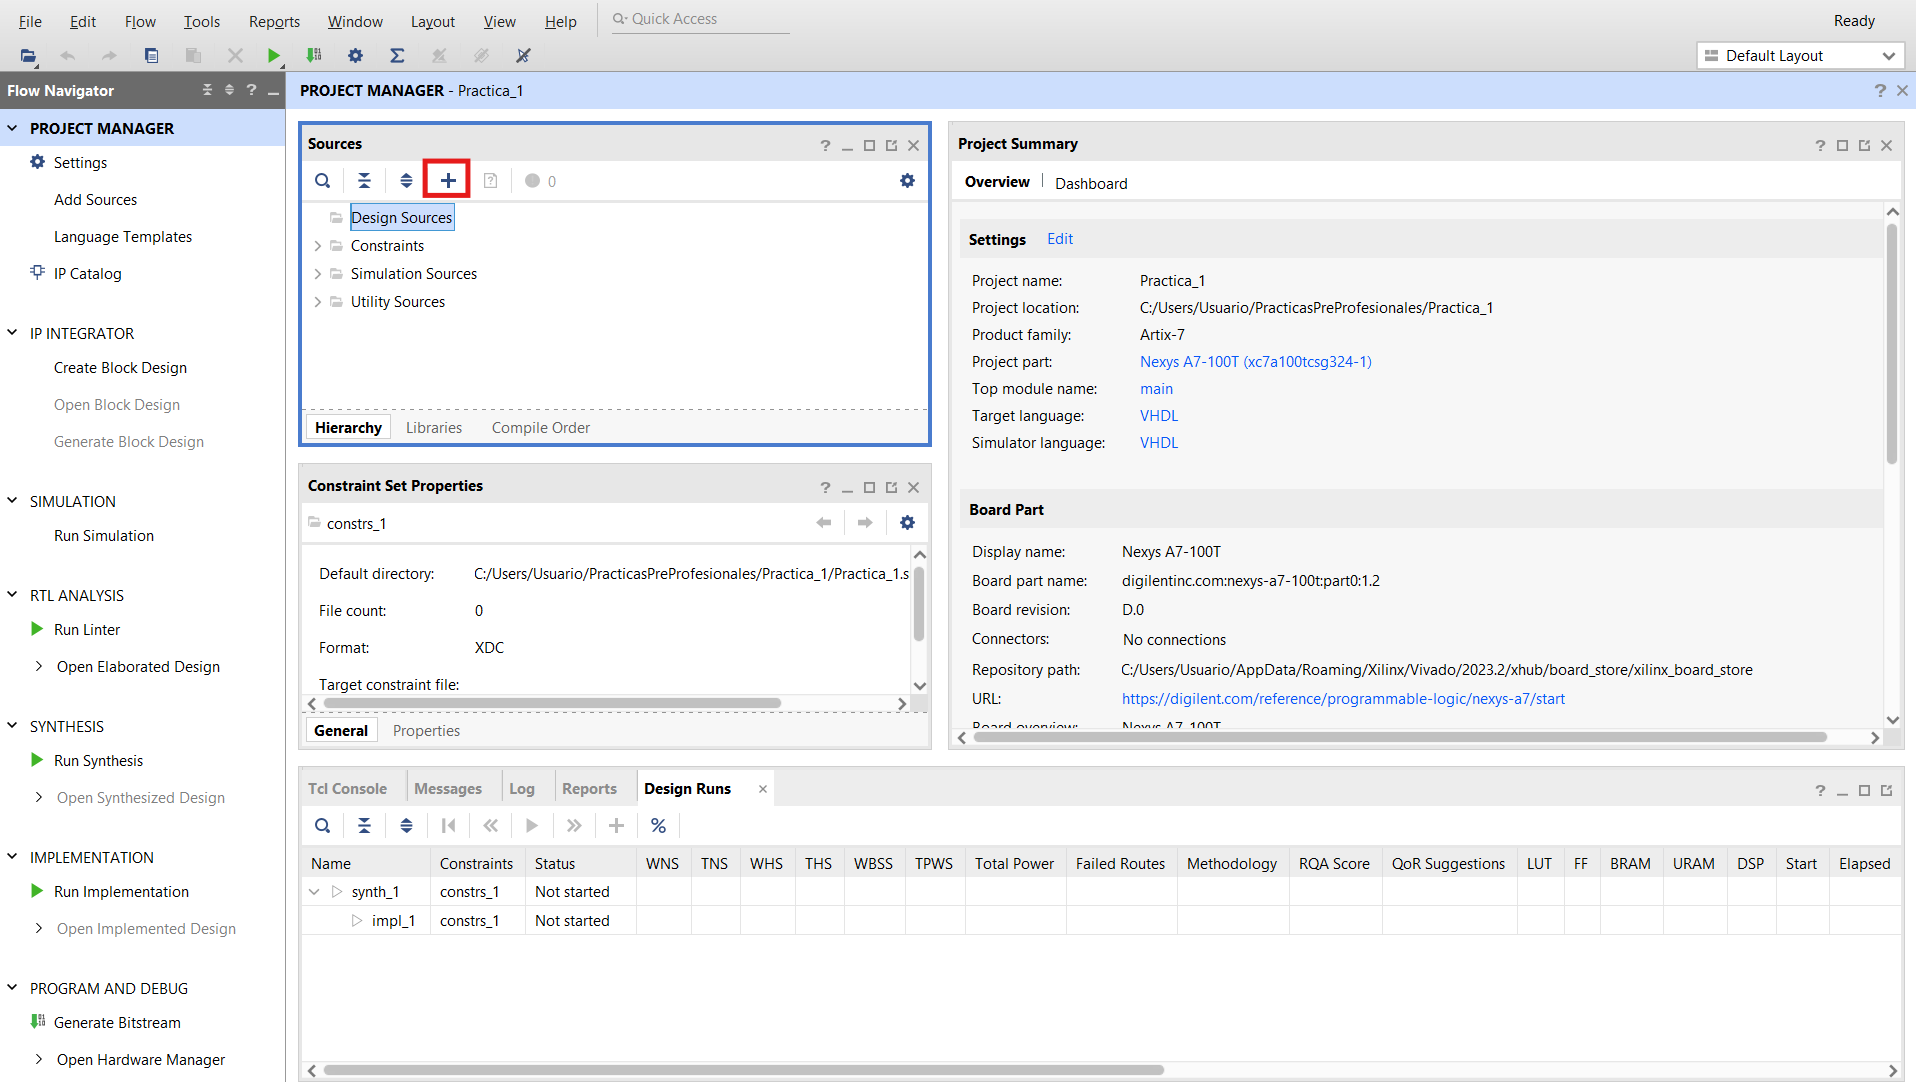
\includegraphics[width=0.8\textwidth]{Creacion_Proyecto/Diseño_proyecto.png}
    \caption{Ubicacion del botón para la creacion del archivo \textbf{.vhd}.}
    \label{fig:diseño}
    \end{figure}

    \item Se verifica la opción 'Add or create design sources' con esto se continua para la creación del archivo

    \begin{figure}[H]
    \centering
    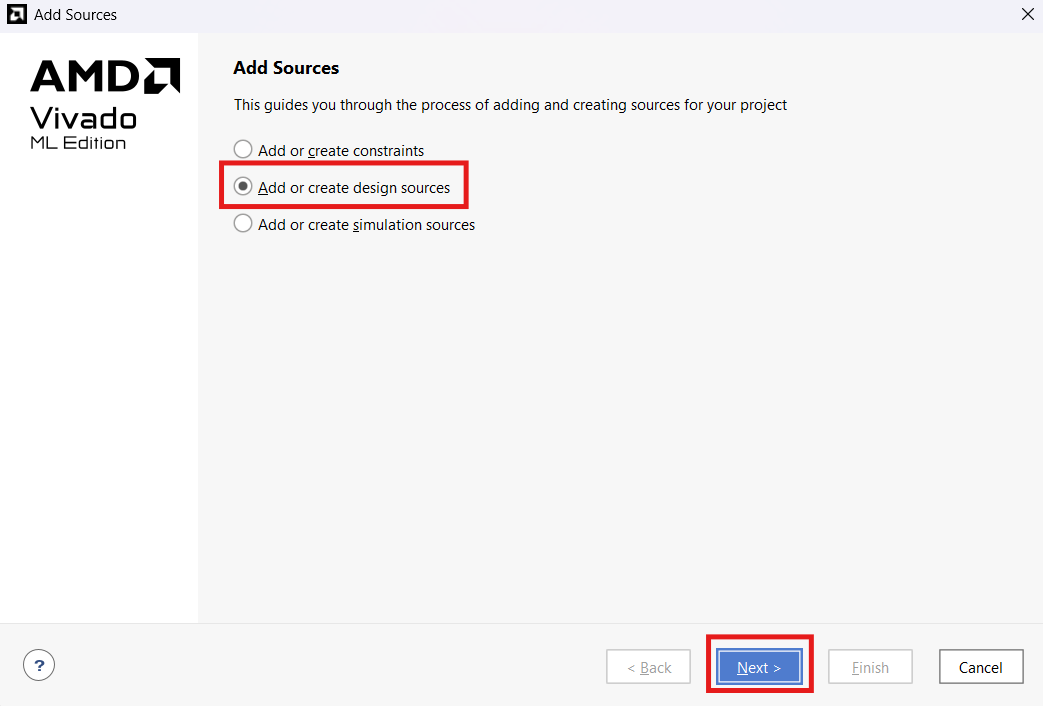
\includegraphics[width=0.8\textwidth]{Creacion_Proyecto/Recursos_proyecto_2.png}
    \caption{Verificación de tipo de recurso a crear.}
    \label{fig:recursos_2}
    \end{figure}

    \item En el siguiente menú se debe seleccionar 'Create File' con ello se abrirá un panel donde se coloca el nombre del archivo a crear, se recomienda el nombre \textbf{main} debido a que se suele usar el nombre main para el archivo principal por analogía con otros lenguajes de programación (como C/C++ o Python), donde main representa el punto de entrada del programa. Aunque en VHDL no existe una función main como tal, este nombre permite identificar rápidamente el módulo que describe el comportamiento principal del circuito.

    \begin{figure}[H]
    \centering
    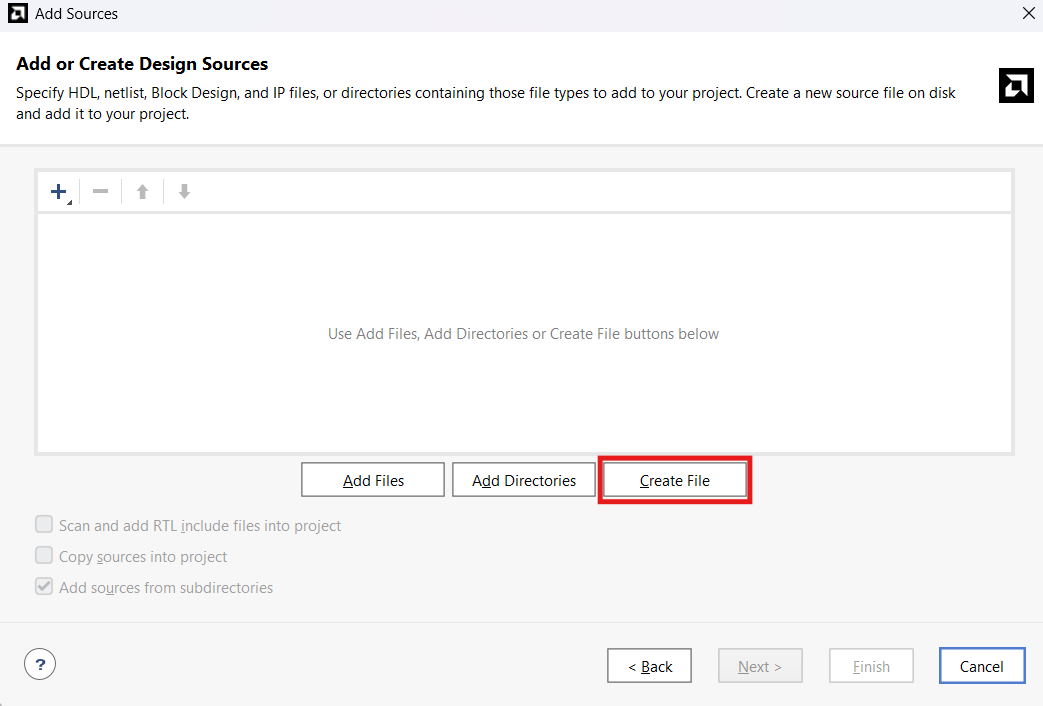
\includegraphics[width=0.8\textwidth]{Creacion_Proyecto/Crear_Archivo_proyecto.png}
    \caption{Manú para la creacion de archivos.}
    \label{fig:recursos_3}
    \end{figure}

    \begin{figure}[H]
    \centering
    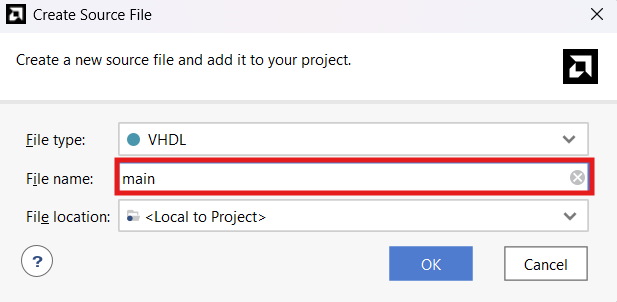
\includegraphics[width=0.8\textwidth]{Creacion_Proyecto/Nombre_archivo_proyecto.png}
    \caption{Nombre del archivo .vhd creado.}
    \label{fig:main}
    \end{figure}

    \item De ser necesario se crean la cantidad de archivos necesarios para cada proyecto, en este caso no es necesario debido a la simpleza del mismo. Una vez finalizado la creación de archivos se finaliza, creando un panel donde se debe En caso de crear un nuevo archivo, especificar el nombre de la
    arquitectura y describir los puertos, este último paso no es
    necesario, se los puede definir por código posteriormente.

    \begin{figure}[H]
    \centering
    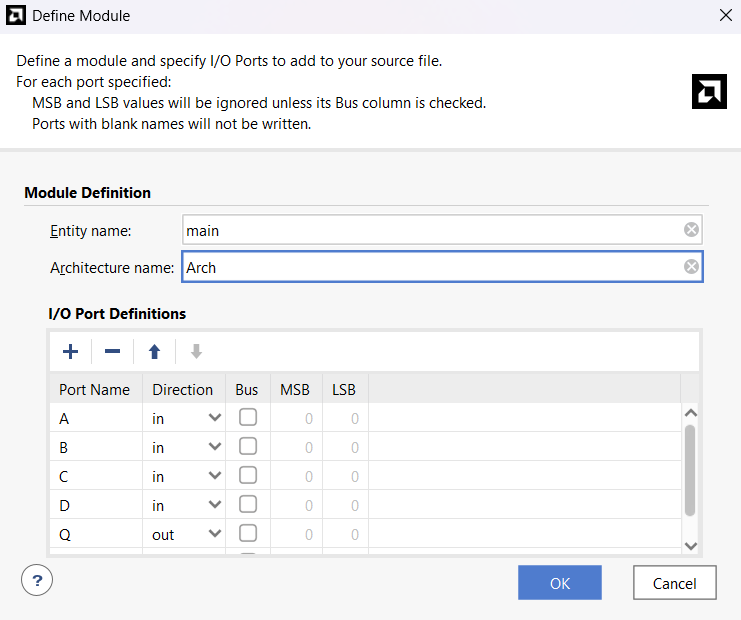
\includegraphics[width=0.8\textwidth]{Creacion_Proyecto/Entradas_proyecto.png}
    \caption{Panel para definir entradas y salidas.}
    \label{fig:i/o}
    \end{figure}

    \item Finalmente para entrar al editor de texto del código en el apartado de \textbf{Design Sources} se debe hacer doble click sobre el archivo creado, en el panel derecho se abre el archivo, de haber especificado las entradas y salidas, estas se crean de manera automática, de lo contrario se deben colocar manualmente

    \begin{figure}[H]
    \centering
    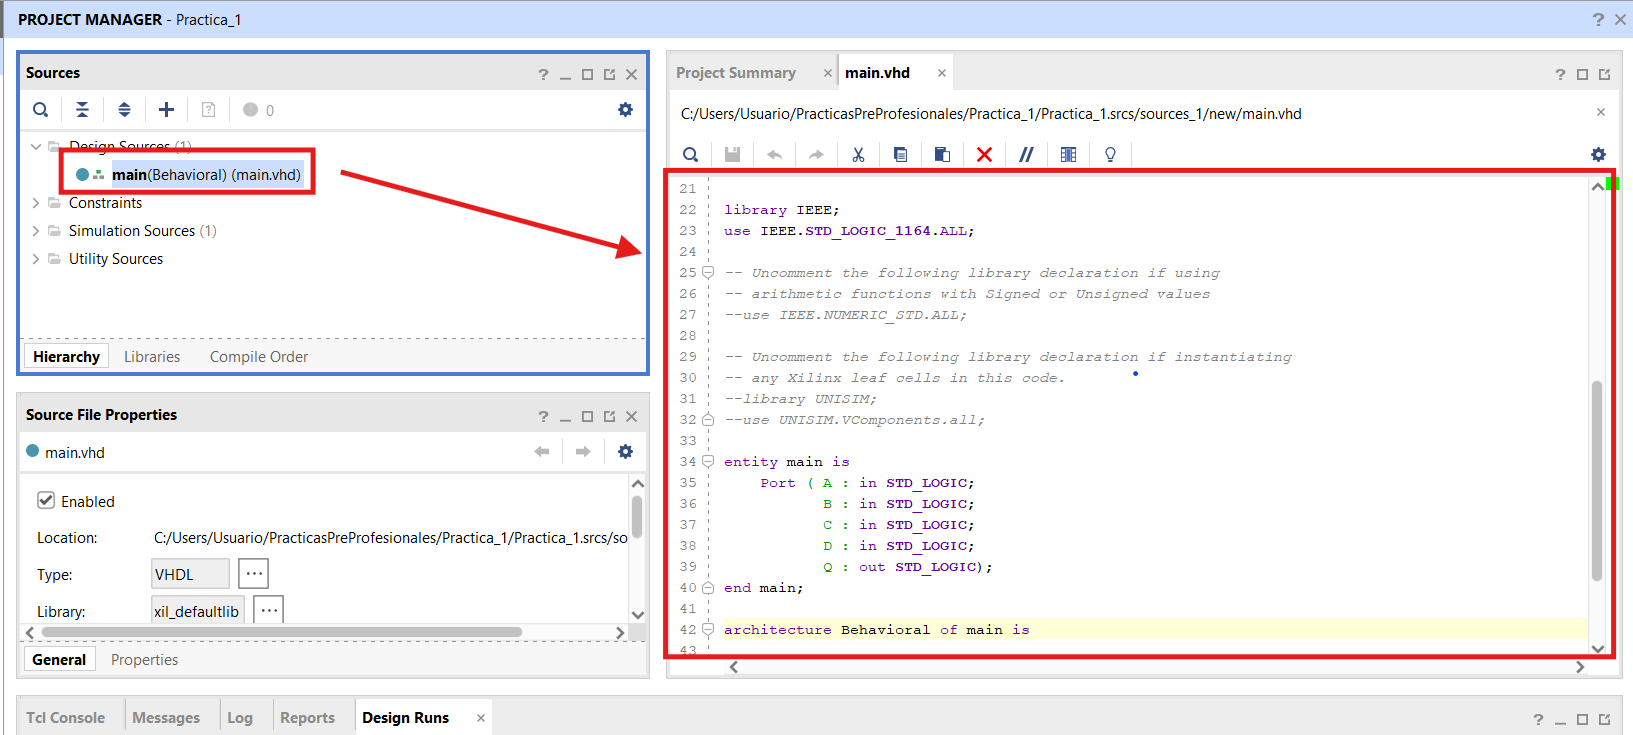
\includegraphics[width=0.8\textwidth]{Creacion_Proyecto/Codigo_proyecto.png}
    \caption{Código main creado.}
    \label{fig:codigo}
    \end{figure}
    
\end{enumerate}

\newpage

\subsection{Creación del módulo VHDL}

Una vez creado el archivo \texttt{.vhd} donde se describirá el comportamiento del circuito se debe comenzar a programar. A continuación se presenta el código VHDL comentado línea por línea, con el objetivo de facilitar su comprensión:

\begin{lstlisting}[caption={Descripción VHDL del circuito combinacional}]
-- Importacion de bibliotecas estandar
library IEEE;
use IEEE.STD_LOGIC_1164.ALL;

-- Declaracion de la entidad
-- La entidad representa la interfaz del circuito: sus entradas y salidas
entity P1circuitocombinacional is
    port (
        A : in std_logic;  -- Entrada A
        B : in std_logic;  -- Entrada B
        C : in std_logic;  -- Entrada C
        D : in std_logic;  -- Entrada D
        Q : out std_logic  -- Salida Q
    );
end P1circuitocombinacional;

-- Arquitectura del circuito
-- Define el comportamiento funcional del circuito descrito en la entidad
architecture Arch of P1circuitocombinacional is
begin
    -- La salida Q se define como: 
    -- (A AND NOT B) XOR NOT(C OR D)
    Q <= (A and (not B)) xor (not (C or D));
end Arch;
\end{lstlisting}


\subsection{Explicación del código}

\begin{itemize}
    \item \textbf{Librerías:} Se importan las librerías estándar del paquete IEEE, particularmente \texttt{STD\_LOGIC\_1164}, que permite el uso de tipos de datos como \texttt{std\_logic}, necesarios para describir señales digitales de uno y cero (y otros estados como 'Z' o 'X').
    
    \item \textbf{Entidad:} La entidad \texttt{P1circuitocombinacional} define los puertos de entrada y salida del módulo. En este caso, se tienen cuatro entradas (\texttt{A, B, C, D}) y una salida (\texttt{Q}), todas de tipo \texttt{std\_logic}.
    
    \item \textbf{Dirección de los puertos:} Se utiliza \texttt{in} para definir entradas, y \texttt{out} para definir salidas. Esto es fundamental para que el compilador del hardware entienda la dirección del flujo de datos.
    
    \item \textbf{Arquitectura:} Bajo el estilo \texttt{Behavioral}, se describe el comportamiento lógico del circuito. Aquí se asigna directamente a la salida \texttt{Q} la expresión booleana requerida, utilizando operadores lógicos estándar de VHDL:
    \begin{itemize}
        \item \texttt{and} → conjunción lógica (AND)
        \item \texttt{or} → disyunción lógica (OR)
        \item \texttt{not} → negación lógica (NOT)
        \item \texttt{xor} → disyunción exclusiva (XOR)
    \end{itemize}
    
    \item \textbf{Asignación concurrente:} La línea que define la salida \texttt{Q} se ejecuta en paralelo con el resto del hardware (no es secuencial), como ocurre en los lenguajes de descripción de hardware.
\end{itemize}

\section{Visualización del esquema RTL (Schematic)}

Una vez completada y guardada la descripción en VHDL, podemos generar automáticamente un esquema lógico del circuito a partir del código fuente. Este esquema nos permite visualizar gráficamente cómo se conectan las señales y cómo se interpreta la arquitectura descrita.

\subsubsection*{Acceso al análisis RTL}

Para ello, realizamos los siguientes pasos dentro del entorno de desarrollo Vivado:

\begin{enumerate}
    \item En el panel de flujo de diseño (Flow Navigator), ubicamos la sección \textbf{RTL Analysis}.
    \item Damos clic en la opción \textbf{Open Elaborated Design}.
    \item Una vez se abra el diseño elaborado, nos dirigimos al menú superior y seleccionamos la opción \textbf{Schematic}.
\end{enumerate}

\begin{figure}[H]
    \centering
    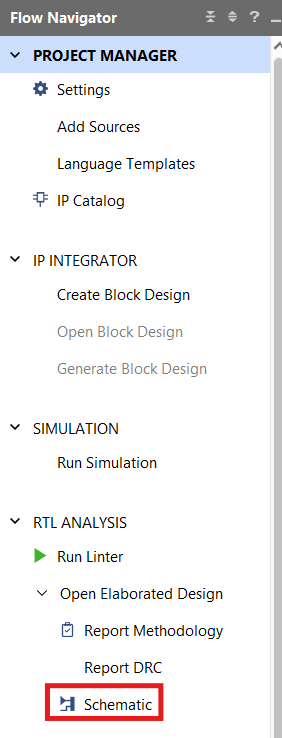
\includegraphics[width=0.45\textwidth]{Implementacion_Proyecto/Esquema.png}
    \caption{Ubicación de la opción \texttt{Open Elaborated Design} en Vivado.}
\end{figure}

\subsubsection*{Interpretación del diagrama generado}

Después de ejecutar estos pasos, Vivado genera automáticamente un esquema que representa la interconexión de los elementos descritos en el archivo VHDL.

\begin{itemize}
    \item Este diagrama muestra los \textbf{puertos de entrada y salida} declarados en la entidad.
    \item Se visualizan también los operadores lógicos y las compuertas que conforman la lógica del circuito combinacional.
    \item Es una herramienta útil para verificar visualmente si el comportamiento programado coincide con la lógica esperada.
\end{itemize}

\begin{figure}[H]
    \centering
    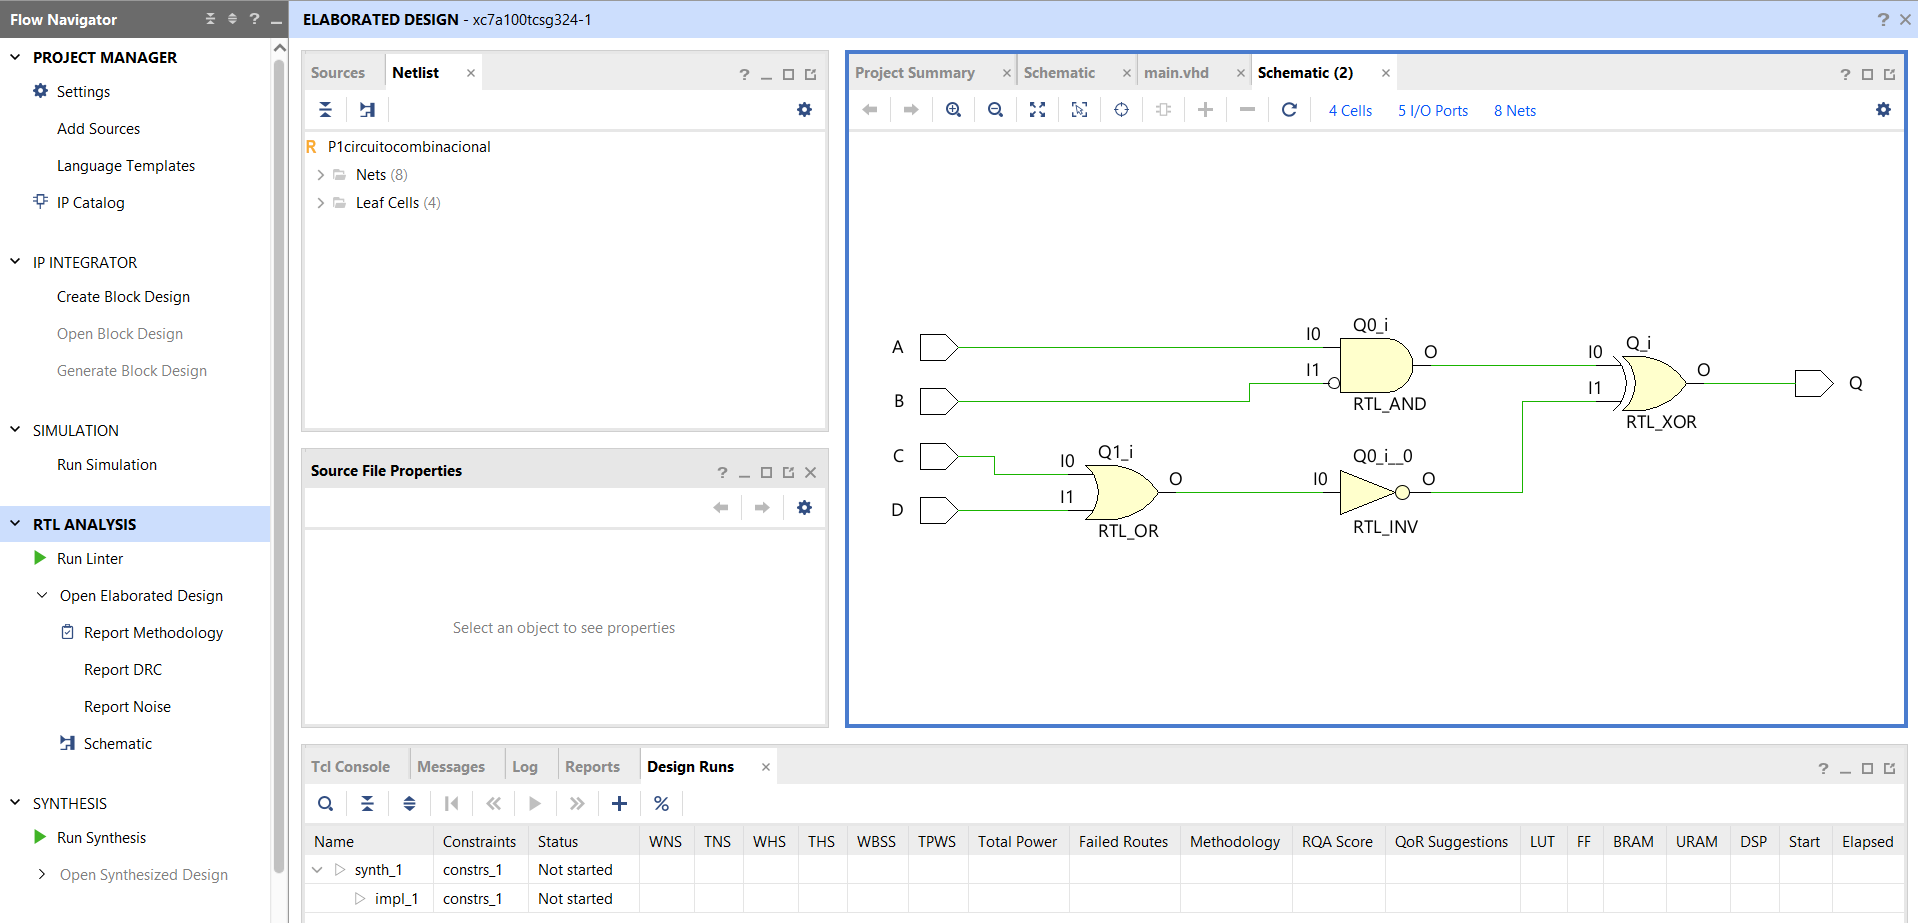
\includegraphics[width=0.85\textwidth]{Implementacion_Proyecto/Diagrama_esquema.png}
    \caption{Esquemático generado automáticamente por Vivado a partir del código VHDL.}
\end{figure}

\begin{quote}
\textbf{Nota:} Es recomendable verificar que las señales estén correctamente conectadas y que la lógica visual refleje la función booleana implementada, como ayuda complementaria a la simulación.
\end{quote}

\section{Asignación de pines de entrada y salida}

Una vez verificado el esquema del circuito, el siguiente paso en el flujo de diseño es la asignación física de los pines de entrada y salida del FPGA. Esta configuración es esencial para vincular correctamente las señales lógicas del código VHDL con los dispositivos físicos de la tarjeta Nexys A7.

\subsubsection{Acceso al panel de pines}

Desde el diseño elaborado en el esquema RTL:

\begin{enumerate}
    \item Damos clic en la opción \textbf{I/O Ports}, ubicada en el margen izquierdo de la vista del esquema.
    \item Se abrirá un panel en la parte inferior del entorno Vivado, donde se listan automáticamente las señales declaradas en la entidad del código VHDL.
\end{enumerate}

\begin{figure}[H]
    \centering
    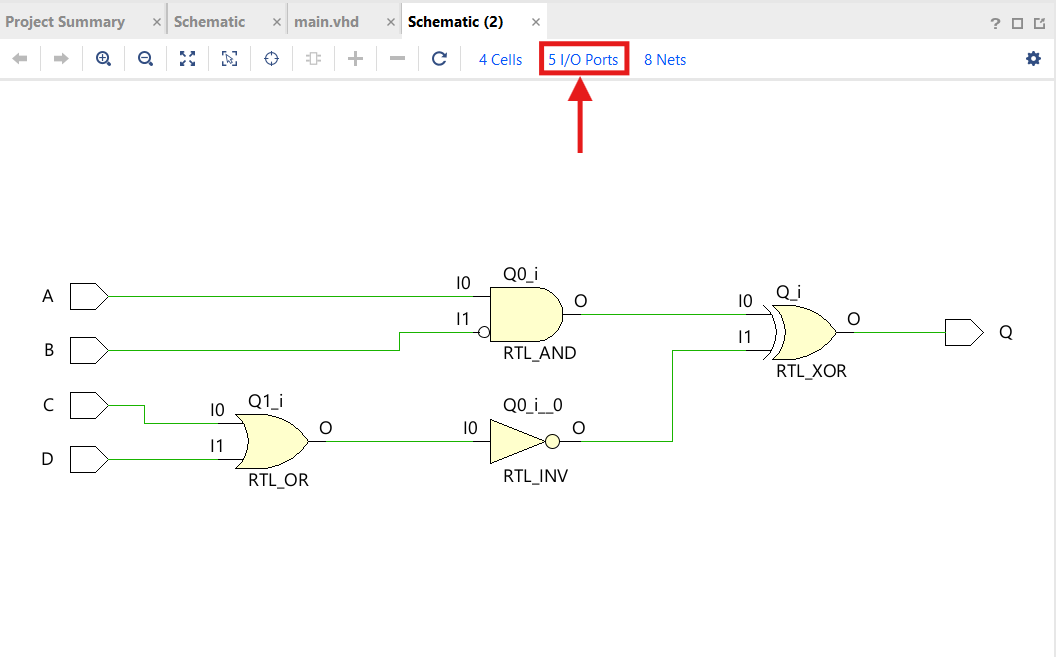
\includegraphics[width=0.8\textwidth]{Implementacion_Proyecto/i_o_puertos.png}
    \caption{Acceso al panel de asignación de puertos (I/O Ports).}
\end{figure}

\subsubsection{Configuración del estándar lógico I/O STD}

En la columna \texttt{I/O Std} del panel de pines, se debe configurar el estándar de voltaje para cada señal. Seleccionamos la opción:

\begin{center}
    \textbf{LVCMOS33}
\end{center}

Este estándar se refiere a la lógica de tipo \textbf{Low Voltage CMOS a 3.3V}, que es el nivel lógico compatible con la mayoría de los periféricos de la placa Nexys A7. Esta configuración asegura que los niveles de voltaje de las señales de entrada y salida se ajusten adecuadamente al hardware físico.

\begin{quote}
\textbf{Nota:} Todos los pines deben tener el mismo estándar lógico, ya que la placa opera con lógica de 3.3V. Usar otro estándar podría causar mal funcionamiento o incluso dañar el FPGA.
\end{quote}

\subsubsection{Asignación de pines físicos (Package Pins)}

Posteriormente, en la columna \texttt{Package Pin}, asignamos manualmente cada una de las señales a su correspondiente pin físico de la tarjeta. En este ejemplo, se realiza la siguiente correspondencia:

\begin{table}[H]
    \centering
    \begin{tabular}{|c|c|c|}
        \hline
        \textbf{Señal VHDL} & \textbf{Pin FPGA} & \textbf{Función en la tarjeta} \\
        \hline
        A & J15 & Switch 0 \\
        B & L16 & Switch 1 \\
        C & M13 & Switch 2 \\
        D & R15 & Switch 3 \\
        Q & H17 & LED 0 \\
        \hline
    \end{tabular}
    \caption{Asignación de señales a pines físicos en la placa Nexys A7.}
\end{table}

\begin{figure}[H]
    \centering
    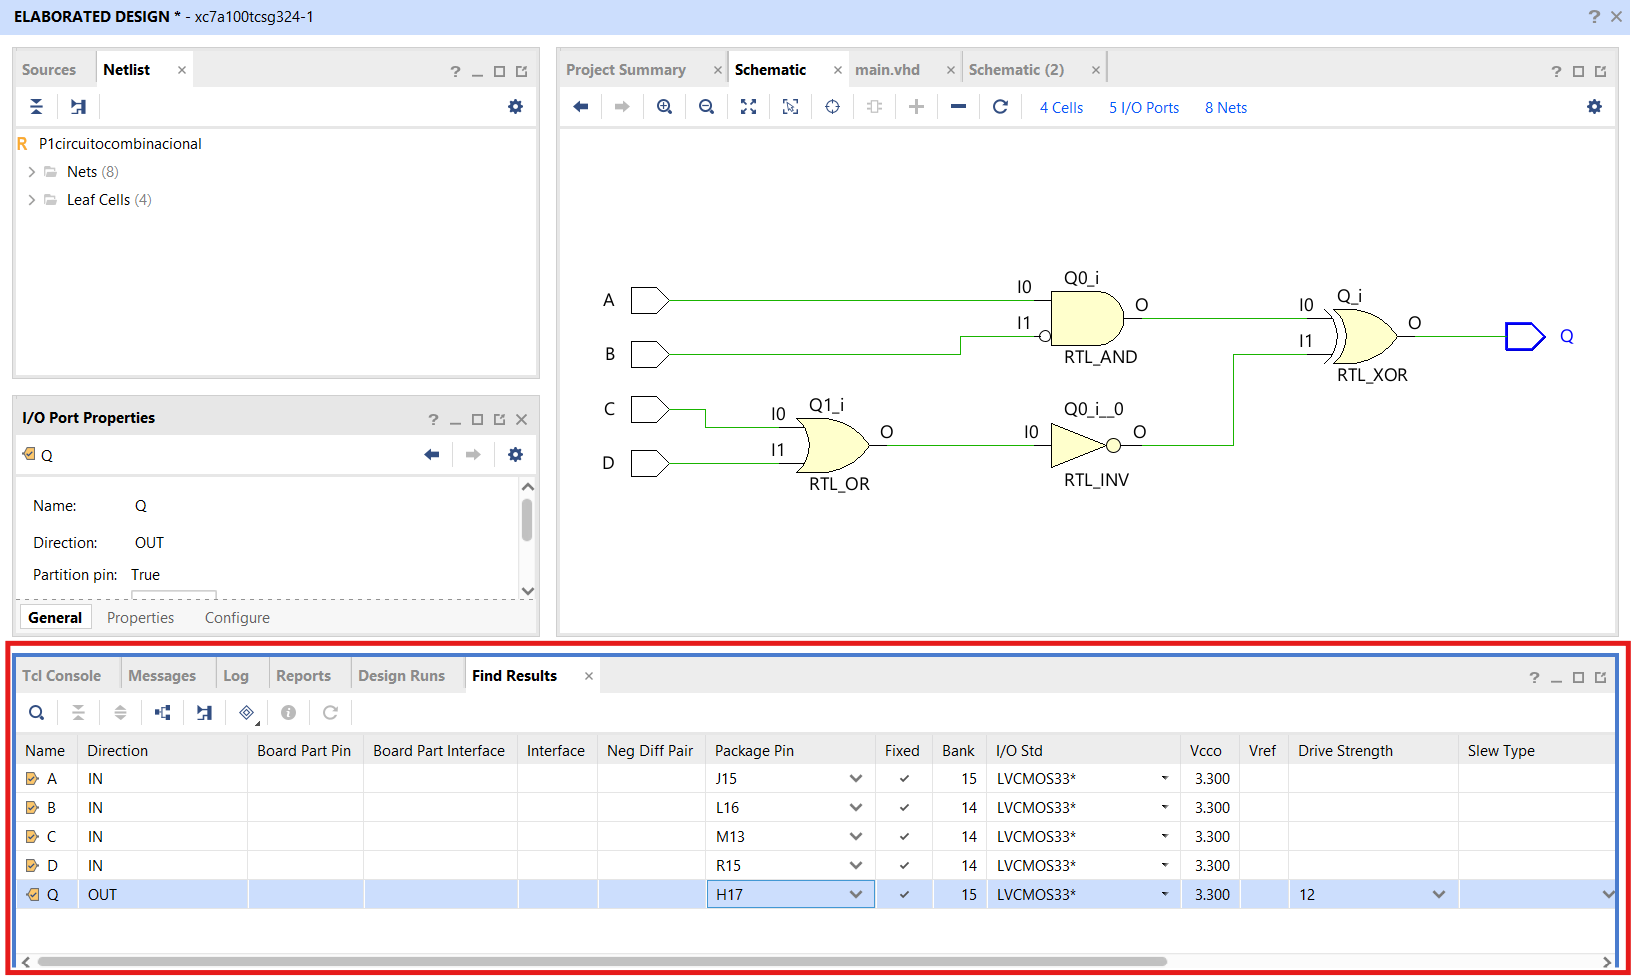
\includegraphics[width=0.95\textwidth]{Implementacion_Proyecto/Pines.png}
    \caption{Vista de asignación de pines en Vivado.}
\end{figure}

\begin{figure}[H]
    \centering
    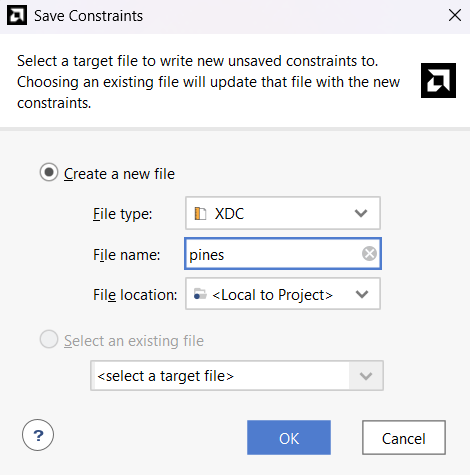
\includegraphics[width=0.75\textwidth]{Implementacion_Proyecto/archivo_pines.png}
    \caption{GUardado del archivo de asignación de pines en Vivado.}
\end{figure}

\subsubsection{Verificación de pines en la documentación de la placa}

Aunque algunos nombres de pines están serigrafiados directamente sobre la placa Nexys A7 (cerca de los switches o LEDs), la verificación más precisa se realiza consultando la \textbf{hoja técnica oficial} (User Guide o Reference Manual) proporcionada por Digilent. En este documento se encuentra el listado completo de los pines y su correspondencia con los periféricos de la placa.

\begin{quote}
\textbf{Recomendación:} Siempre verificar la asignación de pines con el archivo \texttt{.xdc} de referencia que proporciona Digilent para evitar errores de conexión que puedan dañar el FPGA o hacer que el diseño no funcione correctamente.
\end{quote}




\section{Proceso de síntesis, implementación y carga del bitstream en la placa Nexys A7}

Luego de definir el diseño lógico en VHDL y realizar la asignación de pines, el siguiente paso es llevar a cabo la síntesis e implementación del circuito, seguido por la generación y carga del archivo de configuración (\texttt{.bit}) en la FPGA.

\subsection{Synthesis}

El primer paso en el flujo de Vivado es la \textbf{síntesis}.

\begin{itemize}
    \item Se accede a través del menú izquierdo de Vivado, haciendo clic en \textbf{Run Synthesis}.
\end{itemize}

\begin{figure}[H]
    \centering
    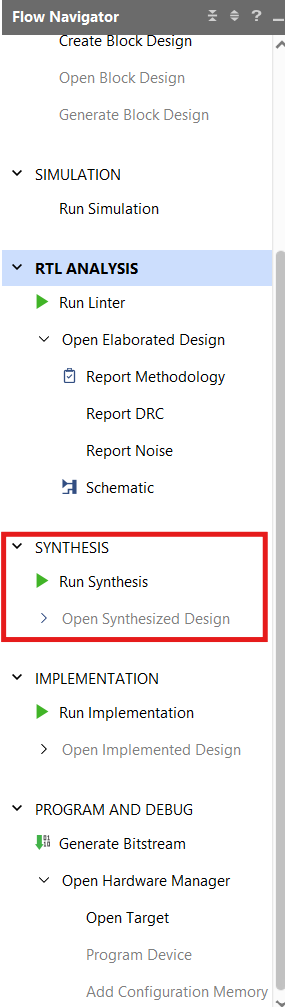
\includegraphics[width=0.25\textwidth]{Implementacion_Proyecto/Synthesis.png}
    \caption{Opción \textit{Run Synthesis} en el flujo de Vivado.}
\end{figure}
\newpage

\paragraph*{¿Qué es la síntesis?}

La síntesis es el proceso mediante el cual el código VHDL es traducido a una representación lógica a nivel de compuertas. Esta etapa convierte las descripciones de alto nivel del comportamiento digital en una red lógica compuesta por LUTs (Look-Up Tables), registros, multiplexores, entre otros.

\paragraph*{Importante:} 
Es fundamental esperar a que la síntesis se complete satisfactoriamente. Al finalizar, se abrirá un panel con varias opciones. En este caso, se debe seleccionar la opción:

\begin{center}
    \textbf{Run Implementation}
\end{center}

\begin{figure}[H]
    \centering
    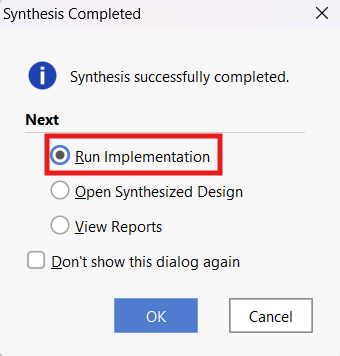
\includegraphics[width=0.5\textwidth]{Implementacion_Proyecto/Synthesis_completa.png}
    \caption{Selección de \textit{Run Implementation} tras la síntesis.}
\end{figure}

\subsection{Implementation}

La implementación, también llamada \textit{place and route}, mapea la lógica sintetizada sobre los recursos físicos de la FPGA, ubicando cada celda lógica, conectándola mediante las rutas disponibles y resolviendo restricciones temporales.

\begin{itemize}
    \item Se ejecuta automáticamente si se seleccionó \textbf{Run Implementation} tras la síntesis, o manualmente desde el menú izquierdo.
\end{itemize}

\paragraph*{¿Por qué es necesaria?}
Este paso garantiza que la lógica se ajuste físicamente a la arquitectura del FPGA, considerando las limitaciones de espacio, temporización y conectividad. Sin esta etapa, no se puede generar un archivo válido de configuración.


Al finalizar la implementación, se abrirá nuevamente un menú. Esta vez, se debe seleccionar la opción:

\begin{center}
    \textbf{Generate Bitstream}
\end{center}

\begin{figure}[H]
    \centering
    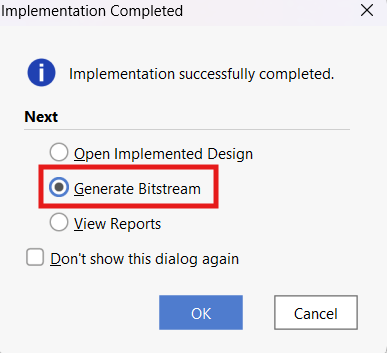
\includegraphics[width=0.65\textwidth]{Implementacion_Proyecto/Implementation.png}
    \caption{Selección de \textit{Generate Bitstream} al finalizar la implementación.}
\end{figure}

\subsection{Generación del Bitstream}

El archivo \texttt{.bit} contiene la información binaria necesaria para programar la FPGA con el diseño implementado. Este archivo configura todos los recursos lógicos internos y define el comportamiento del circuito.

\begin{itemize}
    \item Una vez seleccionada la opción \textbf{Generate Bitstream}, Vivado realiza un empaquetado final.
    \item Al terminar, se muestra un cuadro de confirmación, el cual se puede cerrar sin realizar cambios adicionales.
\end{itemize}

\begin{figure}[H]
    \centering
    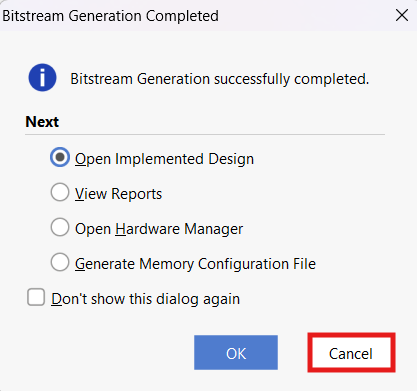
\includegraphics[width=0.65\textwidth]{Implementacion_Proyecto/Bitstream.png}
    \caption{Notificación de bitstream generado.}
\end{figure}

\subsection{Carga del Bitstream en la placa Nexys A7}

Con el archivo \texttt{.bit} generado y la placa Nexys A7 conectada vía USB, se procede a cargar el diseño en el dispositivo FPGA.

\begin{enumerate}
    \item Desde el menú izquierdo, seleccionar \textbf{Open Hardware Manager}.
    \item Luego, hacer clic en \textbf{Open Target} $\rightarrow$ \textbf{Auto Connect}.
    \item Si la placa está correctamente conectada, aparecerá en la lista de dispositivos disponibles.
\end{enumerate}


\begin{enumerate}
    \setcounter{enumi}{3}
    \item Hacer clic derecho sobre el dispositivo detectado y seleccionar \textbf{Program Device}.
    \item Elegir el archivo \texttt{.bit} generado previamente.
    \item Finalmente, presionar \textbf{Program}.
\end{enumerate}

\begin{figure}[H]
    \centering
    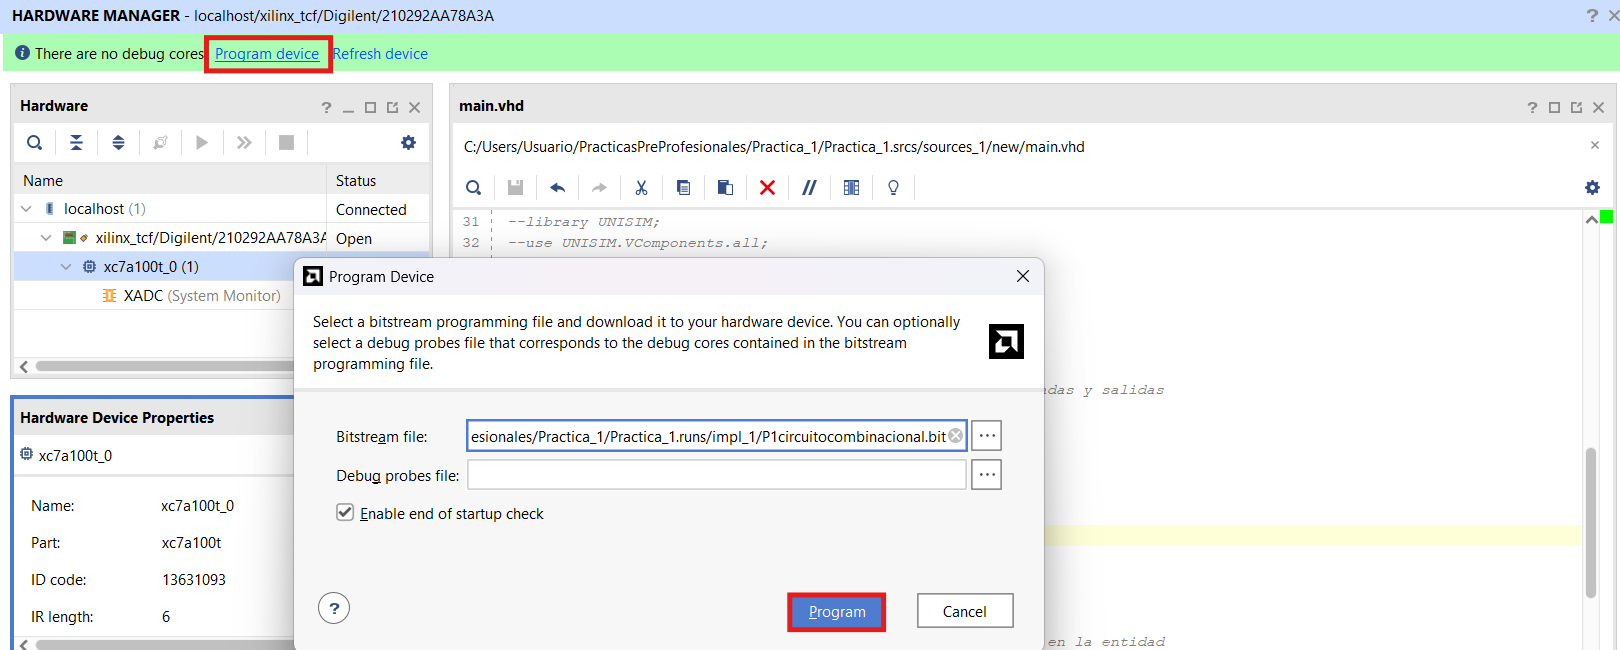
\includegraphics[width=0.7\textwidth]{Implementacion_Proyecto/program.png}
    \caption{Selección del bitstream y programación de la FPGA.}
\end{figure}

\paragraph*{Resultado:} Una vez cargado el bitstream, la FPGA comenzará a ejecutar el diseño configurado. En este caso, los switches conectados a las señales de entrada A, B, C y D afectarán directamente al LED Q, lo cual permite verificar el correcto funcionamiento del diseño implementado.


\section{Resultados en la Placa Nexys}

Una vez cargado correctamente el archivo \texttt{.bit} en la tarjeta de desarrollo Nexys, se puede verificar el funcionamiento del circuito combinacional en tiempo real, utilizando los interruptores (switches) físicos para las entradas \( A \), \( B \), \( C \) y \( D \), y observando el estado del LED correspondiente a la salida \( Q \).

\subsection*{Ejemplos de Combinaciones de Entrada}

En la siguiente tabla se muestran algunos ejemplos específicos de combinaciones aplicadas directamente en la placa, junto con el resultado observado en el LED de salida:

\begin{table}[H]
\centering
\begin{tabular}{|c|c|c|c||c|c|}
\hline
\textbf{A} & \textbf{B} & \textbf{C} & \textbf{D} & \textbf{Expresión Q} & \textbf{LED Encendido} \\
\hline
0 & 0 & 0 & 0 & $(0 \cdot 1) \ \ XOR \ \ (0+0)' = 0 \ \ XOR \ \ 1 = 1$ & Sí \\
\hline
1 & 0 & 1 & 1 & $(1 \cdot 1) \ \ XOR \ \ (1+1)' = 1 \ \ XOR \ \ 0 = 1$ & Sí \\
\hline
1 & 1 & 0 & 0 & $(1 \cdot 0) \ \ XOR \ \ (0+0)' = 0 \ \ XOR \ \ 1 = 1$ & Sí \\
\hline
1 & 1 & 1 & 1 & $(1 \cdot 0) \ \ XOR \ \ (1+1)' = 0 \ \ XOR \ \ 0 = 0$ & No \\
\hline
0 & 0 & 1 & 0 & $(0 \cdot 1) \ \ XOR \ \ (1+0)' = 0 \ \ XOR \ \ 0 = 0$ & No \\
\hline
\end{tabular}
\caption{Resultados observados directamente en la placa Nexys}
\label{tabla_resultados_placa}
\end{table}

\subsection*{Captura Fotográfica del Comportamiento Real}

A continuación se muestran fotografías capturadas durante la ejecución del circuito en la placa Nexys, evidenciando los valores de entrada aplicados mediante los interruptores y el estado del LED indicador de la salida:

\begin{figure}[H]
\centering
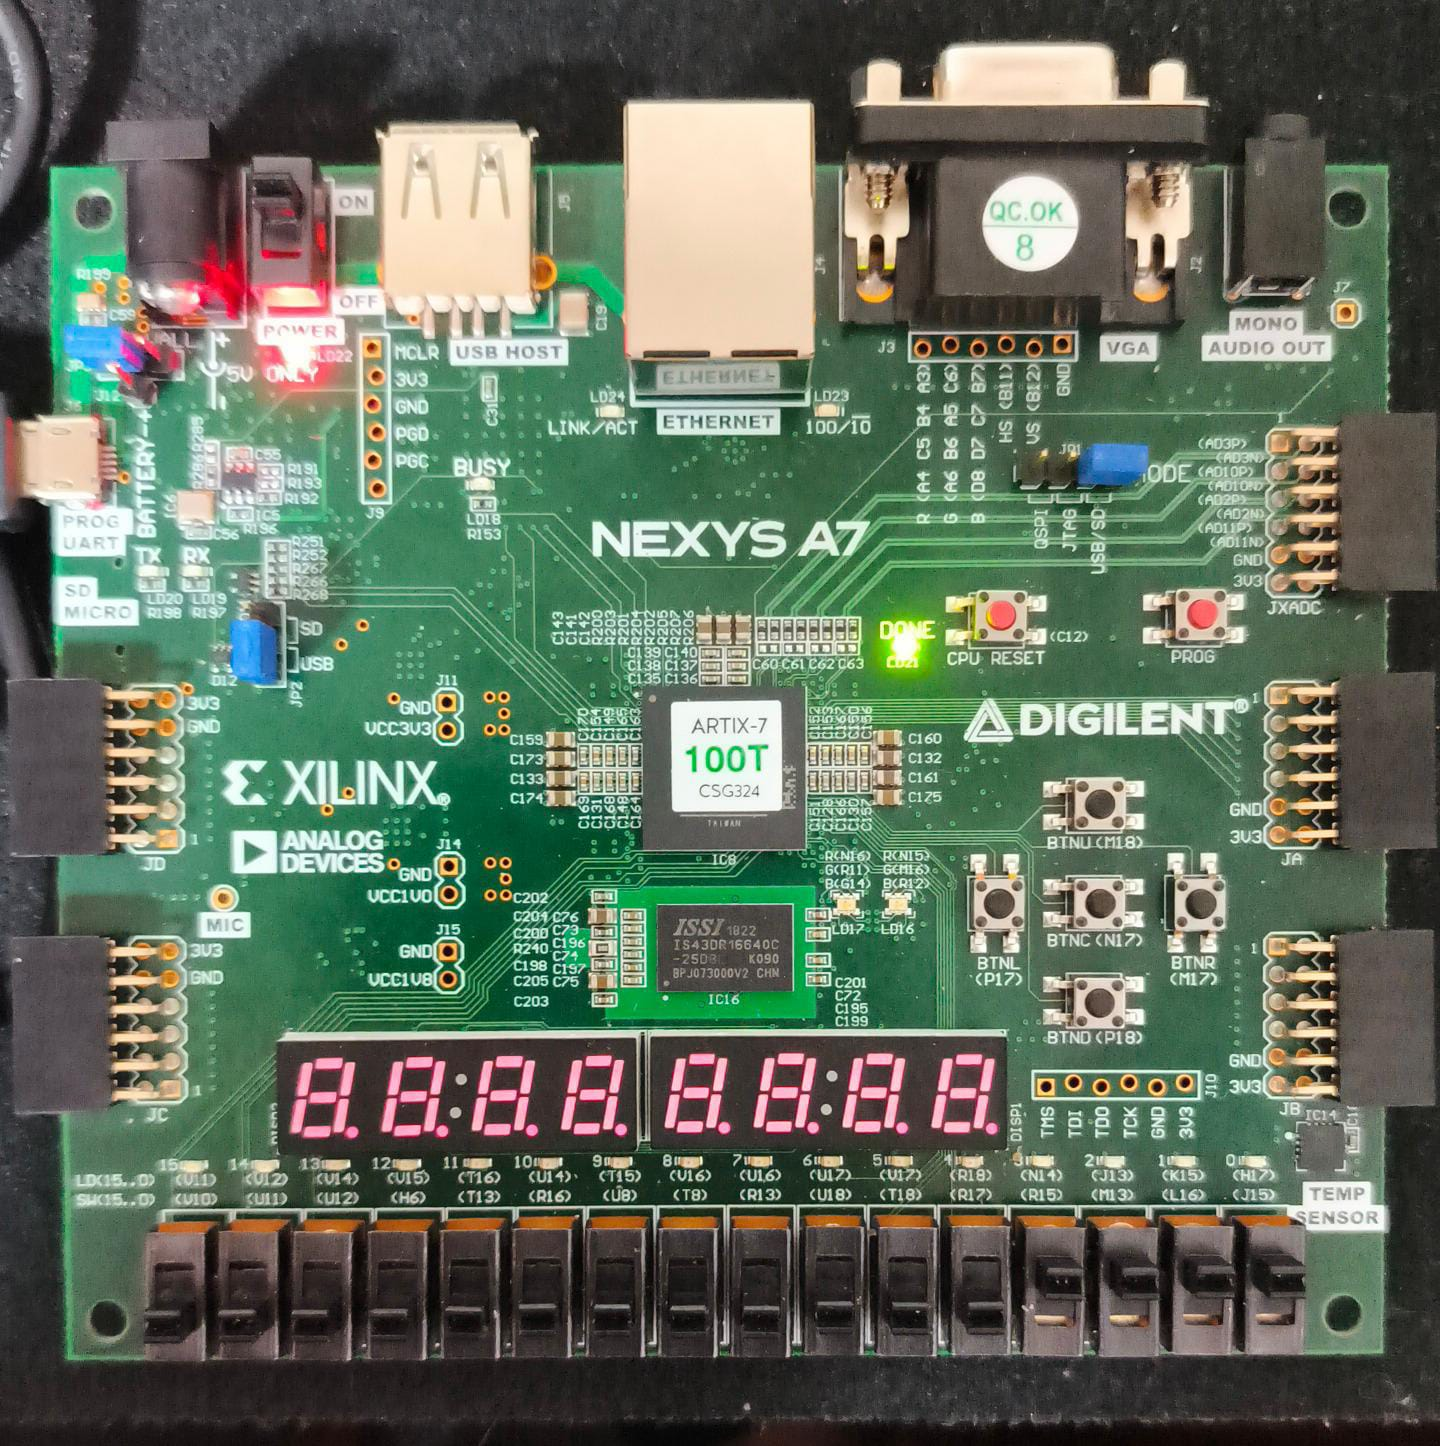
\includegraphics[width=0.65\textwidth]{Implementacion_Proyecto/Salida_0.jpg}
\caption{Combinación A=1, B=1, C=1, D=1. LED apagado (Q=0)}
\end{figure}

\begin{figure}[H]
\centering
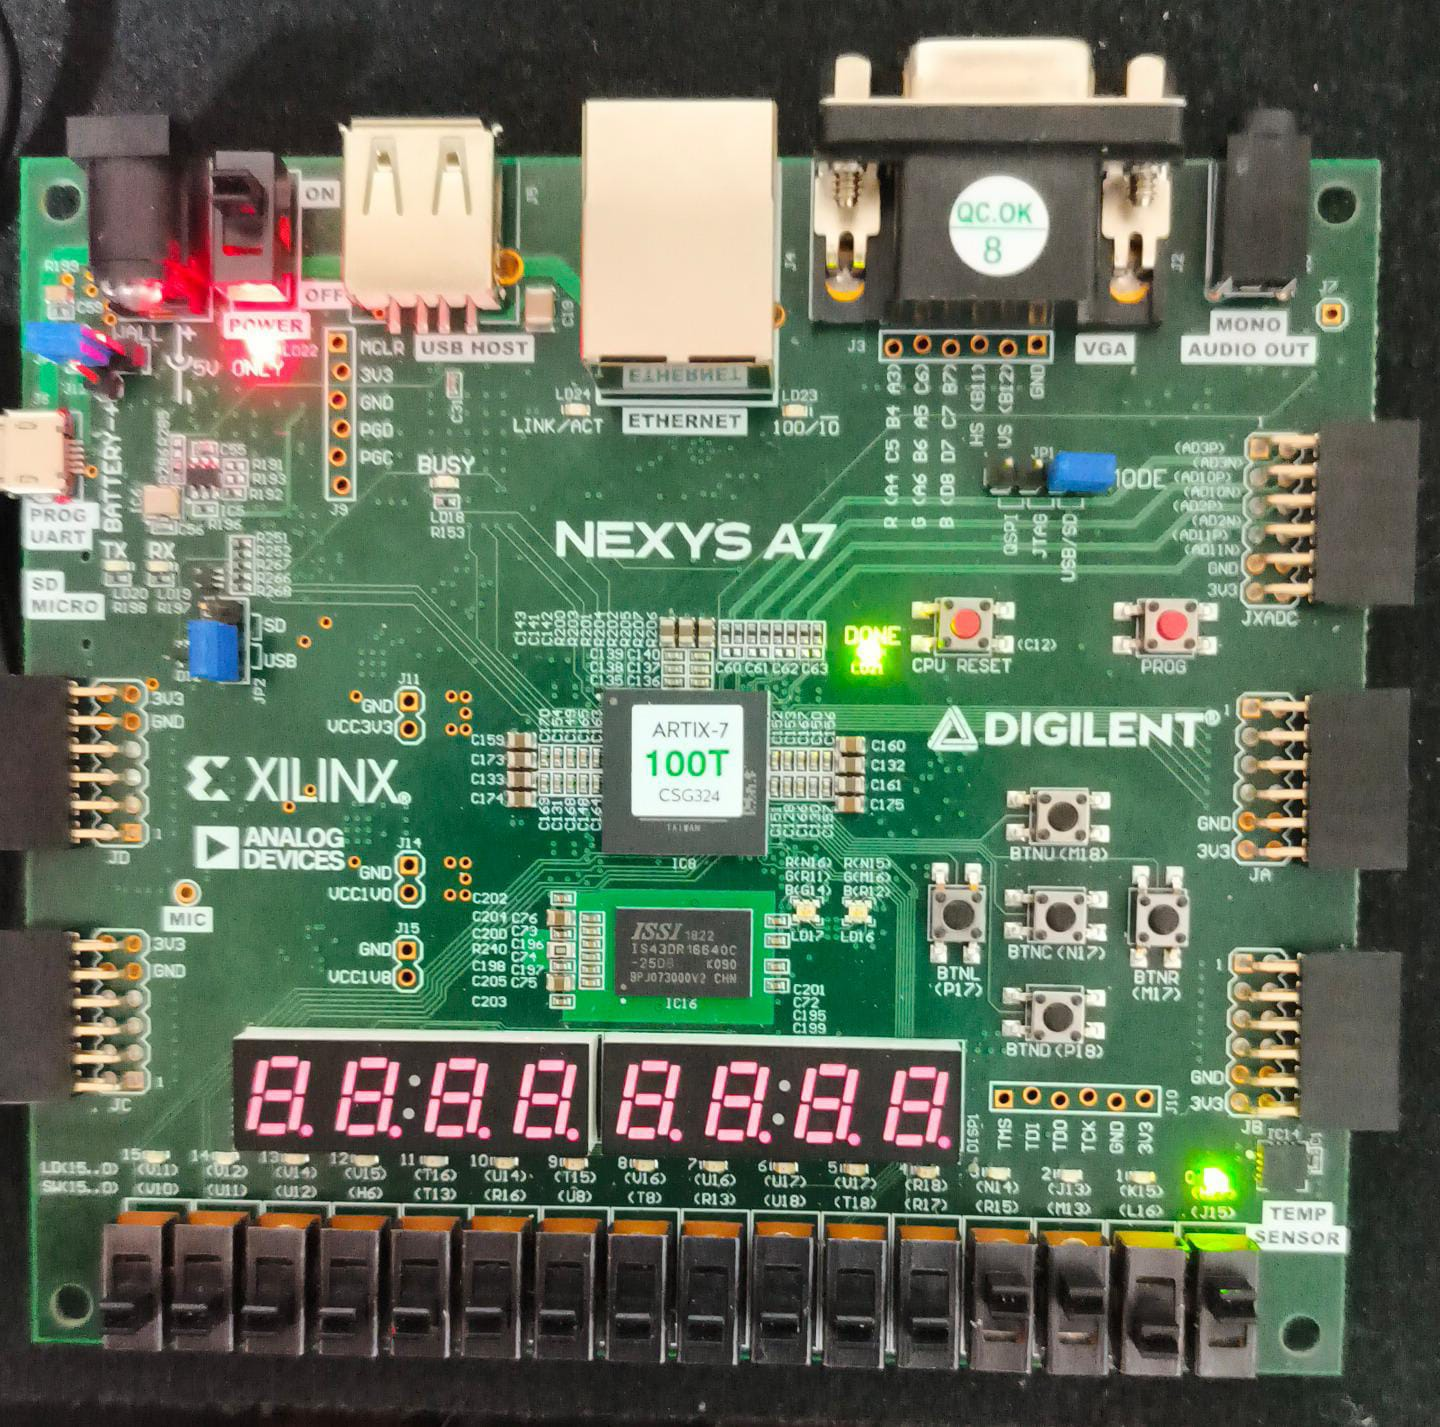
\includegraphics[width=0.65\textwidth]{Implementacion_Proyecto/Salida_1.jpg}
\caption{Combinación A=1, B=0, C=1, D=1. LED encendido (Q=1)}
\end{figure}


\subsection*{Conclusión del Comportamiento Físico}

Se puede concluir que la implementación física en la tarjeta Nexys responde fielmente al diseño lógico planteado en VHDL. Las combinaciones lógicas dadas a través de los switches activan o desactivan el LED de salida conforme a la ecuación implementada:
\[
Q = (A \cdot \overline{B}) \ \ XOR \ \ \overline{(C + D)}
\]
Esto valida que el proceso de síntesis, implementación y asignación de pines fue realizado correctamente.


\end{document}
